\documentclass[11pt,a4paper]{article}

% --- Core Typography & Geometry ---
\usepackage[utf8]{inputenc}
\usepackage[margin=1in]{geometry}
\usepackage{setspace}
\onehalfspacing
\usepackage{microtype}
\usepackage{authblk}

% --- Mathematics & Physics ---
\usepackage{amsmath,amssymb,amsfonts,amsthm}
\usepackage{mathtools}
\usepackage{bm}
\usepackage{braket}

% --- Algorithms & Code ---
\usepackage{algorithm}
\usepackage{algorithmic}

% --- Tables & Floats ---
\usepackage{booktabs}
\usepackage{tabularx}
\usepackage{array}
\usepackage{multirow}
\usepackage{caption}
\usepackage{subcaption}

% --- Graphics & Visuals ---
\usepackage{graphicx}
\usepackage{xcolor}
\usepackage{tikz}
\usetikzlibrary{shapes,arrows,positioning,calc}

% --- Citations & Hyperlinks ---
\usepackage{cite}
\usepackage[colorlinks=true,linkcolor=blue!70!black,citecolor=green!50!black,urlcolor=blue!80!black]{hyperref}

% --- Theorem Environments ---
\newtheorem{theorem}{Theorem}
\newtheorem{lemma}[theorem]{Lemma}
\newtheorem{proposition}[theorem]{Proposition}
\newtheorem{corollary}[theorem]{Corollary}
\theoremstyle{definition}
\newtheorem{definition}{Definition}
\newtheorem{example}{Example}
\theoremstyle{remark}
\newtheorem{remark}{Remark}

% --- Metadata ---
\title{\textbf{\LARGE Quantum-Classical Energy Management and 3D Cyber-Physical Digital Twin Architecture for Priority-Aware Smart Microgrid Optimization}\\[1ex]
\large A Rigorous Multi-Tier Formulation, Variational Algorithmic Benchmark, and Real-Time Spatial Simulation}

\author[1]{\textbf{Vansh Fauzdar}}
\author[2]{\textbf{Nihar Reddy}}
\author[1]{\textbf{Collaborative Research Group in Quantum Systems}}

\affil[1]{Department of Physics and Computational Sciences}
\affil[2]{Department of Electrical Engineering and Smart Grid Systems}
\date{October 2026}

\begin{document}

\maketitle

\begin{abstract}
\noindent The reliable coordination of distributed energy resources (DERs) in decentralized electrical microgrids demands real-time, priority-aware energy dispatch mechanisms capable of preventing catastrophic shedding of life-critical municipal infrastructure during severe generation deficits. This comprehensive study introduces \textbf{QuantumV1}, a unified hybrid quantum-classical optimization architecture and accompanying cyber-physical 3D isometric digital twin environment engineered for autonomous microgrid decision support. We formulate and analyze three mathematically distinct operational regimes: 
\begin{enumerate}
    \item \textbf{Continuous snapshot power dispatch} modeled as a bounded continuous fractional knapsack problem;
    \item \textbf{Indivisible discrete feeder switching} modeled as an NP-hard $0/1$ combinatorial knapsack problem mapped to Quadratic Unconstrained Binary Optimization (QUBO) and solved via the Quantum Approximate Optimization Algorithm (QAOA); and
    \item \textbf{A 24-hour dynamic multi-period dispatch framework} with 218 continuous variables incorporating battery energy storage systems (BESS), solar photovoltaics, and time-of-use tariffs solved via classical linear programming (HiGHS).
\end{enumerate}

Empirical validation was performed across 282 controlled experimental runs spanning seven benchmark campaigns using simulated statevectors with 2,048 projective measurement shots per trial. The QAOA depth sweep demonstrated that advancing variational circuit depth from $p = 1$ to $p = 3$ generated a $74.4\%$ relative increase in optimal ground-state probability mass, achieving a $98.33\%$ ($59/60$) raw-register optimum recovery rate and a $94.44\%$ ($68/72$) ground-state recovery across indivisible switching instances encoded with 5--9 qubits. Conversely, classical mixed-integer linear programming (HiGHS) solved $100\%$ ($50/50$) of scalability benchmark instances up to 200 feeders in an average runtime of $21.3\text{ ms}$, whereas legacy unpruned branch-and-bound exhibited an exponential 1,900-fold runtime increase between 10 and 20 feeders ($3.07\text{ ms}$ to $5,827.09\text{ ms}$). To bridge the operational gap between quantum optimization telemetry and human operators, we architected an interactive, 60 FPS isometric 3D WebGL digital twin employing Three.js, custom GLSL volumetric god-ray shaders, procedural Web Audio synthesis, and bidirectional parameter synchronization. Our findings demonstrate that while classical MILP retains clear practical computational superiority for medium-to-large microgrids in the NISQ era, QAOA provides an effective variational formulation for combinatorial feeder allocation, with the accompanying digital twin establishing a robust, reproducible testbed for future hybrid quantum energy management systems.
\end{abstract}

\vspace{1ex}
\noindent \textbf{Keywords:} Quantum Approximate Optimization Algorithm (QAOA), Quadratic Unconstrained Binary Optimization (QUBO), Microgrid Energy Management, Digital Twin, Three.js, Combinatorial Knapsack, Qiskit, NISQ Benchmarking, HiGHS MILP.

\newpage
\tableofcontents
\newpage

\section{Introduction and Problem Motivation}
\label{sec:intro}

\subsection{Background and Real-World Grid Challenges}
The modern electrical grid is undergoing a fundamental structural transition from centralized, fossil-fueled generation toward decentralized, renewable-dominated architectures. Distributed Energy Resources (DERs)---comprising rooftop and utility-scale photovoltaic (PV) arrays, micro-wind turbines, small-scale run-of-river hydroelectric stations, and Battery Energy Storage Systems (BESS)---form the operational backbone of localized smart microgrids \cite{hirsch2018}. Microgrids offer vital resilience against macro-grid blackouts, support the electrification of remote and rural regions, and diminish aggregate carbon footprints \cite{sharma2022}.

However, the proliferation of DERs introduces profound operational vulnerabilities. Renewable generation is intrinsically stochastic and intermittent, governed by unpredictable meteorological fluctuations such as sudden cloud cover, wind lulls, and seasonal hydrological shifts \cite{thirunavukkarasu2022}. Simultaneously, consumer demand exhibits extreme variability, driven by electric vehicle (EV) charging spikes, industrial machinery duty cycles, and residential thermal regulation. Consequently, microgrid energy management systems (EMS) frequently encounter \textit{generation-deficient operating states}, wherein aggregate instantaneous power demand substantially outstrips local generation and storage discharge capacity \cite{liu2023}.

In physical power systems, persistent supply deficits cause severe frequency dips and voltage instability, which can trigger cascading protective breaker trips and induce total microgrid collapse (blackout). To avert widespread grid failure, the EMS must execute rapid, automated \textit{load shedding} or priority-aware power dispatch \cite{sharma2022}.

\subsection{The Criticality of Priority-Aware Scheduling}
In emergency dispatch regimes, all electrical loads cannot be treated equally. Modern civilized infrastructure relies on a clear hierarchy of societal and operational criticality:
\begin{itemize}
    \item \textbf{Life-Critical Loads (Priority Tier 1):} Regional hospitals, trauma care units, intensive care monitoring, vaccine refrigeration, and emergency response communications. Loss of power introduces an immediate risk to human life.
    \item \textbf{High-Priority Municipal Loads (Priority Tier 2):} Educational institutions, water purification and sewage pumping stations, and municipal police/fire control hubs.
    \item \textbf{Medium-Priority Commercial Loads (Priority Tier 3):} Commercial complexes, smart manufacturing factories, data processing facilities, and EV fast-charging corridors.
    \item \textbf{Low-Priority Residential Loads (Priority Tier 4):} Non-essential residential circuits, decorative municipal illumination, and deferrable domestic heating.
\end{itemize}

When available generation is constrained, an intelligent EMS must allocate power such that unmet demand at high-priority loads incurs heavily penalized costs compared to unserved demand at lower-priority loads. This gives rise to a family of constrained mathematical optimization problems.

\subsection{Continuous vs. Indivisible Combinatorial Allocation}
In the power systems literature, a recurring conceptual ambiguity exists between continuous power throttling and discrete feeder switching:
\begin{enumerate}
    \item \textbf{Continuous Power Allocation:} When individual loads or substations are equipped with local inverters, smart solid-state power electronic transformers, or building automation systems, power delivery $x_i$ can be modulated continuously between $0$ and maximum demand $D_i$. As will be proven in Section~\ref{sec:math_formulations}, this problem reduces to the continuous fractional knapsack problem and can be solved to exact global optimality in $\mathcal{O}(M \log M)$ time using a priority-greedy sorting algorithm.
    \item \textbf{Indivisible Discrete Feeder Switching:} In typical medium- and low-voltage distribution grids, individual feeder breakers operate in binary states: a feeder is either fully energized ($b_i = 1, x_i = D_i$) or fully disconnected ($b_i = 0, x_i = 0$). Partial powering is prohibited because running transformers or motors at severely reduced voltages induces overheating, brownouts, and physical damage. This indivisible switching regime constitutes an NP-hard $0/1$ knapsack problem, where greedy prioritization fails to guarantee global optimality due to volumetric packing inefficiencies.
\end{enumerate}

\subsection{Quantum Optimization Opportunities in the NISQ Era}
As microgrids scale to include hundreds of micro-generators and thousands of addressable switching circuits, the combinatorial search space of $0/1$ feeder assignments scales exponentially as $2^M$. On classical computational architectures, solving large-scale integer programs under strict real-time deadlines (e.g., within 50--100 milliseconds for grid protection relays) can encounter performance bottlenecks \cite{chen2025}.

The advent of Noisy Intermediate-Scale Quantum (NISQ) hardware \cite{preskill2018} has stimulated significant interest in quantum heuristic algorithms. In particular, the Quantum Approximate Optimization Algorithm (QAOA) \cite{farhi2014} maps combinatorial problems formulated as Quadratic Unconstrained Binary Optimization (QUBO) models onto transverse-field Ising spin Hamiltonians. By systematically alternating between problem-specific phase separation unitaries and non-commuting mixer operators, QAOA prepares parameterized variational quantum states whose measurement registers concentrate probability mass around optimal and near-optimal binary configurations.

\subsection{The Cognitive Gap: Cyber-Physical Digital Twins}
While quantum optimization algorithms possess profound theoretical appeal, they are notoriously opaque to power grid operators. Conventional quantum simulators operate as headless command-line scripts or static tabular spreadsheets. In industrial power control centers, operators require intuitive, spatial, real-time cyber-physical representations to visualize grid topology, monitor real-time power flows, inspect qubit allocation weights, and comprehend the physical consequences of quantum optimization decisions.

\subsection{Research Objectives and Scope}
To bridge these fundamental gaps, this paper presents \textbf{QuantumV1}, an integrated quantum-classical energy management framework coupled to a real-time 3D isometric cyber-physical digital twin. The primary objectives of this research are:
\begin{enumerate}
    \item To provide rigorous mathematical formulations and proofs distinguishing continuous fractional knapsack dispatch from discrete $0/1$ feeder switching.
    \item To formulate a mathematically robust QUBO mapping for indivisible feeder switching utilizing dyadic slack variable expansion to strictly enforce inequality capacity constraints.
    \item To implement, simulate, and benchmark QAOA circuits across variational depths $p \in \{1, 2, 3\}$, assessing the impact of circuit depth on ground-state probability mass concentration.
    \item To rigorously evaluate post-measurement classical candidate filtering mechanisms, specifically quantifying the effects of frequency-squared thresholding ($f^2 \ge 10^{-6}$) on production solver hit rates.
    \item To execute an extensive empirical benchmarking campaign encompassing 282 runs across seven controlled test environments, comparing QAOA directly against exact classical Branch-and-Bound and industrial-grade HiGHS Mixed-Integer Linear Programming (MILP).
    \item To engineer a high-performance, 60 FPS 3D isometric WebGL digital twin employing Three.js, volumetric post-processing shaders, procedural audio synthesis, and bidirectional telemetry integration with the quantum optimization engine.
\end{enumerate}


\section{Comprehensive Literature Review and Theoretical Landscape}
\label{sec:lit_review}

\subsection{Decentralized Microgrid Energy Management Systems}
Energy management in microgrids has been an active area of investigation for over two decades. Hirsch et al. \cite{hirsch2018} performed a seminal review of microgrid technologies, delineating the operational drivers that necessitate autonomous local control. Their study underscored that while physical interconnection allows islanded autonomy, it shifts the burden of voltage and frequency stability entirely onto local dispatch controllers. 

Sharma et al. \cite{sharma2022} provided a critical comparative survey of decision-making strategies in microgrid EMS, categorizing methodologies based on centralized, decentralized, and hierarchical control structures. They established that renewable intermittency and stochastic demand profiles invalidate static schedule dispatch, requiring dynamic real-time optimization. Furthermore, Sharma et al. emphasized that when generation is insufficient, priority-weighted load shedding is essential to safeguard critical services.

Thirunavukkarasu et al. \cite{thirunavukkarasu2022} surveyed classical optimization techniques applied to microgrid EMS, analyzing linear programming, mixed-integer linear programming, multi-agent decentralized systems, and metaheuristics (genetic algorithms, particle swarm optimization). They demonstrated that while MILP provides deterministic optimality guarantees through linear relaxations and branch-and-cut routines, computational runtime scales poorly as combinatorial discrete constraints proliferate across extended prediction horizons.

\subsection{Combinatorial Knapsack Complexity in Power Distribution}
The challenge of indivisible feeder switching is isomorphic to the classic $0/1$ knapsack problem, first formulated in combinatorial mathematics by Dantzig \cite{dantzig1957}. In standard complexity theory, the $0/1$ knapsack problem is known to be NP-complete, with its optimization variant being NP-hard \cite{karp1972}. While pseudo-polynomial time dynamic programming algorithms exist ($\mathcal{O}(M S)$ where $S$ is the integer capacity), they become computationally intractable when capacity values are large or continuous.

In power distribution networks, rapid breaker operation requires microsecond-to-millisecond response times. Classical heuristic approximations (such as greedy value-to-weight density ranking) achieve an approximation ratio of $1/2$ for the $0/1$ knapsack problem, meaning that naive greedy heuristics can produce allocations that deviate from the true combinatorial optimum by up to $50\%$. Consequently, exact mathematical programming or advanced heuristic search techniques are mandatory.

\subsection{The Physics of QUBO and Ising Spin Glass Formulations}
Quadratic Unconstrained Binary Optimization (QUBO) has emerged as the universal lingua franca for non-convex combinatorial optimization on quantum devices and classical Ising hardware \cite{glover2019}. A standard QUBO problem seeks to minimize an unconstrained quadratic polynomial over binary decision variables $\mathbf{y} \in \{0, 1\}^N$:
\begin{equation}
\min_{\mathbf{y} \in \{0, 1\}^N} Q(\mathbf{y}) = \sum_{j=1}^N a_j y_j + \sum_{j < k} b_{jk} y_j y_k = \mathbf{y}^T \mathbf{Q} \mathbf{y}
\end{equation}
Because binary variables satisfy the idempotent identity $y_j^2 = y_j$, linear terms are absorbed along the diagonal elements $Q_{jj} = a_j$, while bilinear interaction terms occupy off-diagonal entries $Q_{jk} = b_{jk}$.

The mapping from QUBO to quantum Hamiltonians is grounded in the statistical physics of the Ising spin glass model \cite{lucas2014}. Lucas published a landmark compendium deriving explicit Ising formulations for all of Karp's 21 NP-complete problems, including the knapsack problem, number partitioning, and graph coloring. By executing the canonical affine transformation:
\begin{equation}
y_j \mapsto \frac{I - Z_j}{2}
\end{equation}
where $Z_j = \begin{pmatrix} 1 & 0 \\ 0 & -1 \end{pmatrix}$ is the Pauli-$Z$ operator acting on the Hilbert space of qubit $j$ and $I$ is the $2 \times 2$ identity matrix, binary variables taking values in $\{0, 1\}$ are mapped to quantum spin operators with eigenvalues $\pm 1$:
\begin{equation}
Z_j |0\rangle = +1 |0\rangle, \quad Z_j |1\rangle = -1 |1\rangle
\end{equation}
Under this substitution, products of binary variables transform into tensor products of Pauli operators:
\begin{equation}
y_j y_k \mapsto \frac{I - Z_j}{2} \frac{I - Z_k}{2} = \frac{1}{4} \left( I - Z_j - Z_k + Z_j Z_k \right)
\end{equation}
This substitution maps the classical objective matrix $\mathbf{Q}$ into an equivalent diagonal cost Hamiltonian $H_C$:
\begin{equation}
H_C = C_0 I + \sum_{j=1}^N h_j Z_j + \sum_{j < k} J_{jk} Z_j Z_k
\end{equation}
where $C_0$ represents a scalar energy offset, $h_j$ denotes local magnetic fields, and $J_{jk}$ represents pairwise spin-spin coupling interactions. The ground state (eigenstate corresponding to the minimum eigenvalue) of $H_C$ corresponds exactly to the optimal binary vector $\mathbf{y}^*$ that minimizes the QUBO objective.

\subsection{Quantum Annealing vs. Gate-Based Variational Algorithms}
Two distinct quantum paradigms are utilized to explore Ising ground states:
\begin{enumerate}
    \item \textbf{Quantum Annealing (Adiabatic Quantum Computing):} Implemented physically on specialized analog hardware (e.g., D-Wave flux-qubit processors). The system is initialized in the ground state of a simple transverse-field Hamiltonian and slowly evolved according to the time-dependent Schr{\"o}dinger equation toward $H_C$. By the Adiabatic Theorem, if the evolution time $T$ is sufficiently long ($T \gg \frac{1}{\Delta_{\min}^2}$, where $\Delta_{\min}$ is the minimum instantaneous spectral gap), the system remains in the ground state throughout the trajectory.
    \item \textbf{Gate-Based Variational Algorithms (QAOA):} Implemented on universal, gate-model quantum computers (e.g., superconducting transmons, trapped ions). Farhi, Goldstone, and Gutmann \cite{farhi2014} introduced QAOA as a discretization of adiabatic evolution into an alternating sequence of parameterized quantum logic gates. Unlike analog annealers, gate-based QAOA allows precise circuit depth control, software-defined mixer Hamiltonians, and compatibility with universal error-mitigated gate architectures.
\end{enumerate}

\subsection{Variational Quantum Optimization in Electrical Power Systems}
The deployment of variational quantum algorithms within electrical power engineering has accelerated rapidly. Koretsky et al. \cite{koretsky2021} adapted QAOA to generator unit commitment (UC), converting quadratic fuel cost curves and minimum-up/down operational constraints into QUBO form. While they demonstrated successful circuit compilation, they established that classical commercial solvers (such as CPLEX and Gurobi) remained vastly superior for instances with fewer than 400 generation units.

Liu and Tang \cite{liu2023} provided a foundational tutorial on quantum computing for power systems, reviewing applications across power flow, state estimation, fault diagnosis, and contingency analysis. They emphasized that the quadratic overhead of slack variable expansion often inflates the required qubit register count beyond the physical capacity of current NISQ chips.

Chen and Vu \cite{chen2025} of Pacific Northwest National Laboratory (PNNL) authored an exhaustive technical report detailing quantum algorithms across transmission and distribution grids. They highlighted the critical necessity of qubit-efficient encoding schemes (such as logarithmic basis representations) to mitigate hardware bottleneck constraints.

Ajagekar and You \cite{ajagekar2019} evaluated quantum computing for energy systems optimization, showing that hybrid classical-quantum loops frequently encounter severe non-convex optimization challenges during parameter estimation, including barren plateaus where cost function gradients vanish exponentially with qubit count.

Liu et al. \cite{liu2025} investigated QAOA for decentralized microgrid scheduling, demonstrating that priority weighting can be embedded directly into penalty functions. In parallel, the multi-institutional Q-GRID project summarized by Blenninger et al. \cite{blenninger2024} established standard benchmarking protocols for quantum grid optimization, issuing a strong methodological warning: claims of quantum utility or advantage cannot be made without rigorous comparisons against modern, multi-threaded classical MILP baselines.


\section{Cyber-Physical Co-Simulation: 3D Digital Twin and Quantum Dashboard}
\label{sec:twin_and_dashboard}

The \textbf{QuantumV1} framework bridges the cognitive and operational divide between abstract variational quantum algorithms and physical distribution grid operations via a tightly coupled, dual-module cyber-physical co-simulation architecture. As illustrated in Figure~\ref{fig:co_simulation_arch}, the platform comprises two synchronized operational layers:
\begin{enumerate}
    \item \textbf{The Physical Spatial Twin (Module 1):} A high-performance, 60~FPS isometric 3D WebGL engine running in the browser (\texttt{http://localhost:8080}), providing volumetric visual feedback, transmission routing, diurnal cycles, and physical asset interaction.
    \item \textbf{The Analytical Quantum Dashboard (Module 2):} An interactive Python/Streamlit computational cockpit (\texttt{http://localhost:8501}) powered by Qiskit Aer and SciPy HiGHS, hosting the QUBO synthesis pipeline, variational circuit transpiler, measurement histogram inspector, and longitudinal empirical benchmark repository.
\end{enumerate}

\begin{figure*}[t]
\centering
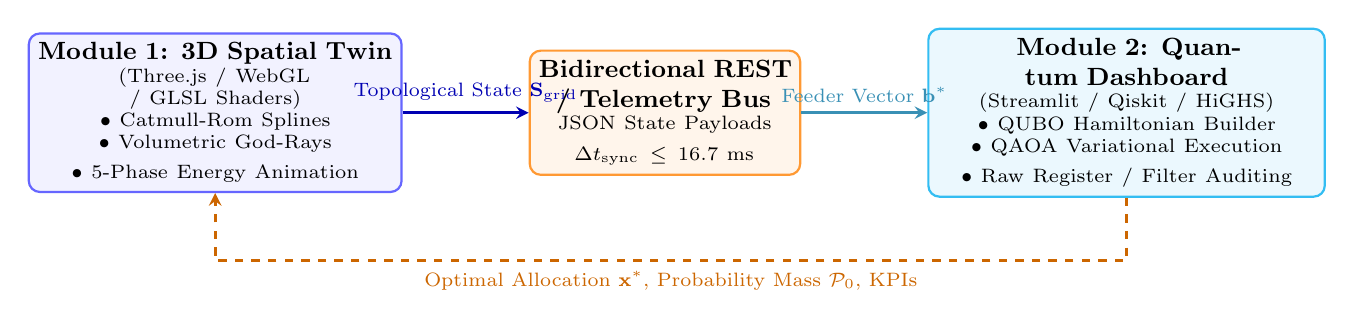
\begin{tikzpicture}[
    node distance=1.5cm,
    block/.style={rectangle, draw=blue!60, fill=blue!5, thick, text centered, rounded corners, minimum height=1.1cm, minimum width=3.4cm, font=\small},
    qblock/.style={rectangle, draw=cyan!80, fill=cyan!8, thick, text centered, rounded corners, minimum height=1.1cm, minimum width=3.4cm, font=\small},
    cblock/.style={rectangle, draw=orange!80, fill=orange!8, thick, text centered, rounded corners, minimum height=1.1cm, minimum width=3.4cm, font=\small},
    arrow/.style={thick, ->, >=stealth}
]
    % Module 1: 3D Twin
    \node[block, text width=4.5cm] (twin) {\textbf{Module 1: 3D Spatial Twin}\\\scriptsize (Three.js / WebGL / GLSL Shaders)\\$\bullet$ Catmull-Rom Splines\\$\bullet$ Volumetric God-Rays\\$\bullet$ 5-Phase Energy Animation};
    
    % Synchronization Bus
    \node[cblock, right=1.6cm of twin, text width=3.2cm] (bus) {\textbf{Bidirectional REST / Telemetry Bus}\\\scriptsize JSON State Payloads\\$\Delta t_{\text{sync}} \le 16.7\text{ ms}$};
    
    % Module 2: Dashboard
    \node[qblock, right=1.6cm of bus, text width=4.8cm] (dash) {\textbf{Module 2: Quantum Dashboard}\\\scriptsize (Streamlit / Qiskit / HiGHS)\\$\bullet$ QUBO Hamiltonian Builder\\$\bullet$ QAOA Variational Execution\\$\bullet$ Raw Register / Filter Auditing};

    % Connections
    \draw[arrow, line width=1pt, color=blue!70!black] (twin.east) -- node[above, font=\scriptsize] {Topological State $\mathbf{S}_{\text{grid}}$} (bus.west);
    \draw[arrow, line width=1pt, color=cyan!70!black] (bus.east) -- node[above, font=\scriptsize] {Feeder Vector $\mathbf{b}^*$} (dash.west);
    \draw[arrow, line width=1pt, dashed, color=orange!80!black] (dash.south) -- ++(0,-0.8) -| node[near start, below, font=\scriptsize] {Optimal Allocation $\mathbf{x}^*$, Probability Mass $\mathcal{P}_0$, KPIs} (twin.south);
\end{tikzpicture}
\caption{Bidirectional Co-Simulation Architecture between the 3D Cyber-Physical Spatial Twin (\texttt{localhost:8080}) and the Analytical Quantum Energy Dashboard (\texttt{localhost:8501}).}
\label{fig:co_simulation_arch}
\end{figure*}

\subsection{Module 1: 3D Cyber-Physical Spatial Digital Twin}
\label{subsec:3d_twin}

The spatial digital twin is rendered natively in modern web browsers without external plugins using WebGL via the \textbf{Three.js} framework. The scene graph represents an isolated rural smart-grid diorama housing distributed generation sources (Solar PV, Wind Turbine, Small Hydro Dam, and Battery Energy Storage System [BESS]) and priority-stratified municipal loads (Memorial Medical Center, Oakridge Community Academy, Metro Corporate Commercial, and Greenfield Residential).

\begin{figure*}[t]
\centering
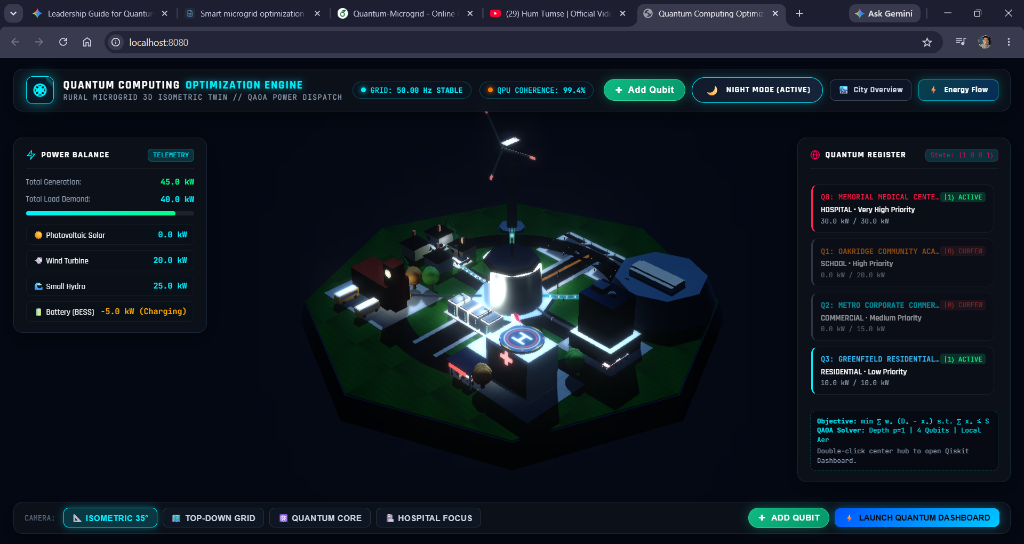
\includegraphics[width=0.96\textwidth]{figures/fig_twin_3d_night.png}
\caption{The 3D Cyber-Physical Spatial Digital Twin (\texttt{http://localhost:8080}) rendered in nocturnal operating mode. Key elements include the central illuminated substation QPU node, Catmull-Rom spline conduits displaying photon flow, the live power balance telemetry panel ($45.0\text{ kW}$ generation vs. $40.0\text{ kW}$ load with $-5.0\text{ kW}$ BESS charging), and the reactive Quantum Register HUD confirming feeder states $|1\,0\,0\,1\rangle$ (Hospital [30.0 kW] and Residential [10.0 kW] active, School and Commercial placed on night curfew).}
\label{fig:twin_3d_night}
\end{figure*}

\subsubsection{Visual Shader Pipeline and Volumetric Atmospheric Scattering}
To achieve photorealistic visual fidelity while maintaining stable 60~FPS execution, the rendering pipeline employs a multi-pass \texttt{EffectComposer}:
\begin{itemize}
    \item \textbf{Dual-Pass Selective Bloom (\texttt{UnrealBloomPass}):} Emissive transmission conduits, transformer bushings, and coherent QPU conduits exceed a tuned luminance high-pass threshold ($L_{\text{thresh}} = 0.85$ night, $0.90$ day). Luminescent bloom ($\text{strength} = 1.20$, $\text{radius} = 0.55$) is blended additively, rendering branch power loading with vivid neon glow.
    \item \textbf{Screen-Space Volumetric God-Rays (\texttt{godrays.js}):} Daytime atmospheric shafts are synthesized via a custom screen-space radial blur shader. Projecting the sun's 3D position into normalized device coordinates $\mathbf{s}_{\text{sun}} \in [-1, 1]^2$, the shader accumulates 100 attenuated samples along the screen-space ray:
    \begin{equation}
    I_{\text{godray}}(\mathbf{u}) = \frac{1}{K} \sum_{k=0}^{K-1} \gamma^k \cdot \mathcal{T}\left(\mathbf{u} - k \cdot \frac{\mathbf{u} - \mathbf{s}_{\text{sun}}}{K} \cdot \delta\right)
    \end{equation}
    where $\mathcal{T}$ represents the occluder buffer, $\gamma = 0.96$ is the attenuation decay factor, and $\delta = 0.85$ is the ray density step.
\end{itemize}

\subsubsection{Dynamic Diurnal Cycles and Kinetic Camera Physics}
The digital twin features an interactive diurnal engine and kinetic navigation system:
\begin{itemize}
    \item \textbf{Diurnal Light & UI Theme Adaptation:} The solar position traverses an orbital trajectory $\mathbf{p}_{\text{sun}}(t) = [R \cos(\omega t), R \sin(\omega t) \sin(\theta), R \sin(\omega t) \cos(\theta)]^T$. In Night Mode (as shown in Figure~\ref{fig:twin_3d_night}), ambient illumination drops to obsidian twilight populated by 1,400 twinkling star particles, and the glowing AR power lines shift to saturated electric crimson and cobalt blue for optimal legibility.
    \item \textbf{Precision Smart Zoom:} Rather than zooming towards the arbitrary world origin, continuous raycasting detects bounding intersections on infrastructure meshes. When the operator zooms into an asset, the camera focal point smoothly translates towards the target centroid:
    \begin{equation}
    \mathbf{T}_{\text{orbit}}(t + \Delta t) = \mathbf{T}_{\text{orbit}}(t) + \alpha \left( \mathbf{P}_{\text{node}} - \mathbf{T}_{\text{orbit}}(t) \right)
    \end{equation}
    with exponential damping $\alpha = 0.08$, automatically recentering when zooming out to macro level.
\end{itemize}

\subsubsection{Five-Phase Cinematic Energy Flow Visualization}
To convey complex quantum dispatch results, the digital twin executes a timed, 5-phase visual sequence across Catmull-Rom spline conduits (Algorithm~\ref{alg:energy_flow}):
\begin{enumerate}
    \item \textbf{Phase 1: Generation Inception ($0.0 - 3.0\text{ s}$):} Generation nodes (Hydro, Solar, Wind) pulse in electric blue ($P_{\text{gen}} = 80.0\text{ kW}$ total).
    \item \textbf{Phase 2: Quantum Core Processing ($3.0 - 5.5\text{ s}$):} The central Substation Control Center radiates a holographic shockwave, simulating QAOA variational optimization.
    \item \textbf{Phase 3: Conduit Routing ($5.5 - 7.8\text{ s}$):} Photon packets travel along Catmull-Rom spline curves at velocities proportional to power flow ($v_i \propto x_i^*$).
    \item \textbf{Phase 4: Node Fulfillment \& Shedding ($7.8 - 11.0\text{ s}$):} Critical nodes (Hospital, $w_0 = 1000$) illuminate in solid green indicating full fulfillment; non-essential nodes dim to red if shed by the quantum solver ($\mathbb{I}_{\text{shed}} = 1$).
    \item \textbf{Phase 5: Steady-State Transition ($11.0 - 16.0\text{ s}$):} Visual telemetry gently stabilizes into persistent monitoring mode.
\end{enumerate}

\begin{algorithm}[H]
\caption{Five-Phase Cyber-Physical Energy Flow Animation}
\label{alg:energy_flow}
\begin{algorithmic}[1]
\REQUIRE Dispatch vector $\mathbf{x}^* \in \mathbb{R}^M$, Switching vector $\mathbf{b}^* \in \{0, 1\}^M$, Elapsed time $t$.
\ENSURE Spline luminescence $L_i(t)$, Particle velocity $v_i(t)$, Node color $\mathbf{C}_i(t)$.
\IF{$0.0 \le t < 3.0$}
    \STATE $\forall j \in \text{Generators}: \text{PulseLuminance}(j, \text{period}=1.2\text{ s})$.
\ELSIF{$3.0 \le t < 5.5$}
    \STATE $\text{TriggerQPUHologram}(\text{center}=\text{Substation}, \text{radius}=15\text{ m})$.
\ELSIF{$5.5 \le t < 7.8$}
    \FORALL{$i \in \text{Feeders}$}
        \STATE $v_i \leftarrow v_{\text{base}} \cdot (x_i^* / D_i) \cdot b_i^*$
        \STATE $\text{AdvancePhotonParticles}(\text{Spline}_i, v_i)$
    \ENDFOR
\ELSIF{$7.8 \le t < 11.0$}
    \FORALL{$i \in \text{Nodes}$}
        \STATE $\mathbf{C}_i \leftarrow (b_i^* == 1) \;?\; \text{VividGreen} : \text{ShedCrimson}$
        \STATE $\text{SetEmissiveGlow}(\text{Mesh}_i, \mathbf{C}_i)$
    \ENDFOR
\ELSE
    \STATE $\text{NormalizePersistentTelemetry}()$
\ENDIF
\end{algorithmic}
\end{algorithm}

\subsubsection{In-Situ Qubit Customization (\texttt{+ Add Qubit})}
The digital twin functions as an active control console rather than a passive display. Operators can dynamically deploy new archetypes into the grid, including Industrial Smart Factories ($25\text{ kW}$), Quantum AI Data Centers ($35\text{ kW}$), EV Fast-Charging Hubs ($25\text{ kW}$), and Water Treatment Plants ($18\text{ kW}$). Clicking any node opens an in-situ modal to adjust priority weights ($w_i$), nominal power demand ($D_i$), and operational hours (`24/7` vs. daytime work windows).

\subsection{Module 2: Analytical Quantum Optimization Dashboard}
\label{subsec:quantum_dashboard}

Module 2 provides the analytical counterpart to the 3D twin, structured into three dedicated Streamlit cockpits:

\begin{figure}[htbp]
\centering
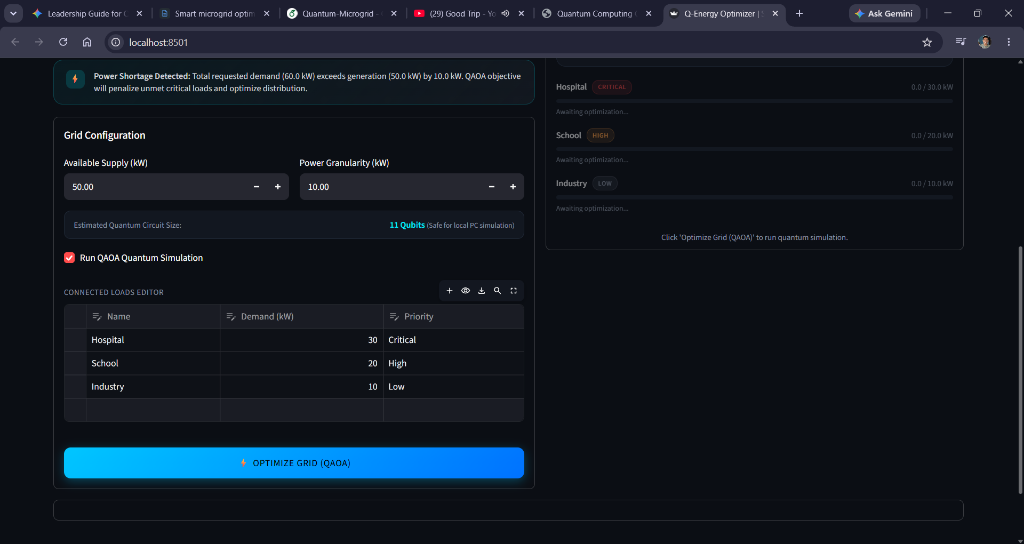
\includegraphics[width=\columnwidth]{figures/fig_dashboard_config.png}
\caption{Quantum Energy Optimizer configuration console (\texttt{http://localhost:8501}). Operators configure generation supply ($50.00\text{ kW}$), power discretization granularity ($10.00\text{ kW}$), and inspect the 11-qubit circuit scale estimation required for dyadic slack encoding across connected loads (Hospital, School, Industry).}
\label{fig:dashboard_config}
\end{figure}

\subsubsection{Cockpit 1: Real-Time Simulation and Configuration Console}
As shown in Figure~\ref{fig:dashboard_config}, the configuration console empowers grid dispatchers to parameterize generation capacity and demand requirements:
\begin{itemize}
    \item \textbf{Deficit Warning Notification:} When aggregate requested demand ($\sum D_i = 60.0\text{ kW}$) exceeds available generation ($S = 50.0\text{ kW}$) by $10.0\text{ kW}$, the engine flags a power shortage and configures the QAOA objective to penalize unmet critical loads.
    \item \textbf{Qubit Register Estimator:} Given power granularity $g = 10.00\text{ kW}$ and supply $S = 50.00\text{ kW}$, the dashboard computes the required binary slack expansion and warns operators of circuit footprint ($N_{\text{qubits}} = 11\text{ qubits}$), confirming safe local statevector execution.
    \item \textbf{Connected Loads Editor:} Dynamic tabular interface allowing dispatchers to edit load priorities (`Critical', `High', `Low') and nominal power draws.
\end{itemize}

\begin{figure}[htbp]
\centering
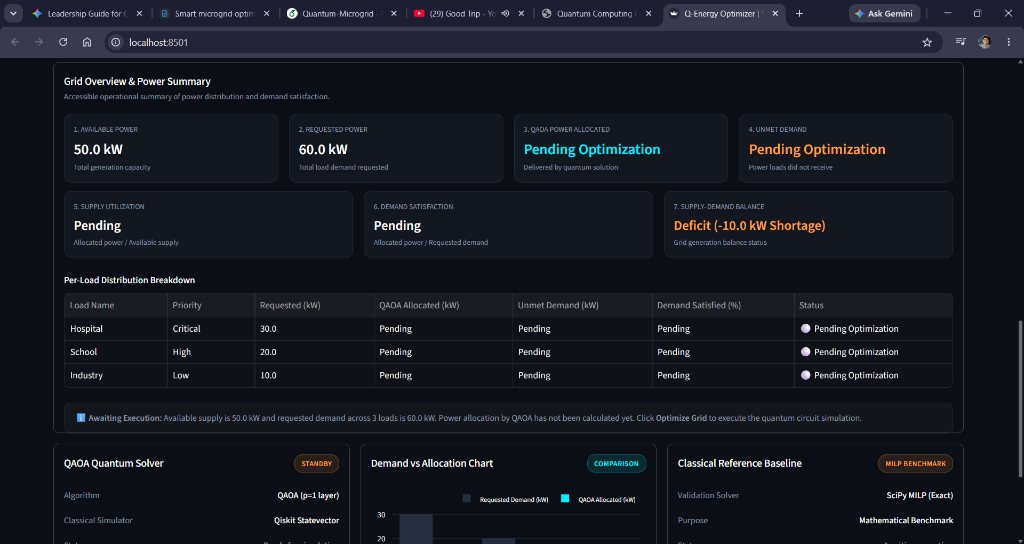
\includegraphics[width=\columnwidth]{figures/fig_dashboard_kpis.png}
\caption{Analytical Quantum Dashboard operational cockpit (\texttt{http://localhost:8501}). Real-time telemetry monitors the 7 primary KPI chips, detects supply deficits ($-10.0\text{ kW}$ shortage), tracks per-load distribution fulfillment, and initializes the dual execution pipeline pitting variational QAOA against the SciPy HiGHS MILP exact classical baseline.}
\label{fig:dashboard_kpis}
\end{figure}

\subsubsection{Cockpit 2: Operational Telemetry & Comparative Dispatch Engine}
As illustrated in Figure~\ref{fig:dashboard_kpis}, Cockpit 2 monitors real-time system performance across seven dedicated KPI chips:
\begin{equation}
S = 50.0\text{ kW}, \quad D_{\text{total}} = 60.0\text{ kW}, \quad \Delta_{\text{margin}} = -10.0\text{ kW (Deficit)}
\end{equation}
Key diagnostic components include:
\begin{itemize}
    \item \textbf{Tri-Solver Comparative Dispatch Engine:} Computes instantaneous power allocations simultaneously across: (a) Continuous Fractional Greedy ($\mathcal{O}(M \log M)$); (b) Classical HiGHS MILP (exact branch-and-cut); and (c) Quantum QAOA ($p \in [1, 5]$). Side-by-side waterfall charts visualize allocation disparities and unserved penalties.
    \item \textbf{Variational Execution Inspector:} Visualizes the COBYLA parameter optimization trajectory $\langle \psi(\boldsymbol{\gamma}, \boldsymbol{\beta}) | H_C | \psi(\boldsymbol{\gamma}, \boldsymbol{\beta}) \rangle$ across optimization steps, confirming classical convergence.
    \item \textbf{Candidate Pool Filtering and Register Auditing:} To prevent classical post-processing defects from discarding valid quantum solutions, Cockpit 2 exposes the complete measurement audit against the frequency-squared threshold:
    \begin{equation}
    \mathcal{C} = \left\{ \mathbf{y} \in \{0, 1\}^N \;\middle|\; \left(\frac{c(\mathbf{y})}{N_{\text{shots}}}\right)^2 \ge \tau = 10^{-6} \right\}
    \end{equation}
    The interface renders a high-resolution Plotly histogram charting the full $2^N$ measurement probability distribution, with feasibility flags ($\sum D_i b_i \le S$) and objective scores $J(\mathbf{y})$ for every measured bitstring.
\end{itemize}

\subsubsection{Cockpit 3: Research Experimentation and Benchmark Repository}
Cockpit 3 hosts the empirical archive of all 282 experimental benchmark runs recorded across seven campaigns:
\begin{itemize}
    \item \textbf{Multi-Dimensional Filtering:} Filters historical runs by solver type, feeder count ($M \in [3, 200]$), circuit depth ($p \in [1, 5]$), and penalty multiplier $P$.
    \item \textbf{Scalability Analytics:} Renders interactive scatter and box plots comparing runtime scaling between QAOA, unpruned B\&B, and HiGHS, demonstrating classical superiority at scale and isolating QAOA probability concentration.
\end{itemize}

\subsection{Bidirectional Telemetry Schema and Co-Simulation Protocol}
\label{subsec:telemetry_schema}

The synchronization between the 3D twin and the quantum calculator occurs over HTTP REST via structured JSON telemetry payloads. Table~\ref{tab:telemetry_schema} outlines the data schema.

\begin{table}[htbp]
\centering
\caption{Bidirectional Telemetry Data Schema Between 3D Twin and Quantum Dashboard}
\label{tab:telemetry_schema}
\renewcommand{\arraystretch}{1.2}
\begin{tabularx}{\columnwidth}{l l X}
\toprule
\textbf{Field} & \textbf{Data Type} & \textbf{Physical Interpretation / Description} \\
\midrule
\texttt{supply\_total} & Float ($\text{kW}$) & Aggregate power from Hydro, Solar PV, Wind, and BESS. \\
\texttt{qubit\_nodes} & Array[Object] & List of loads containing ID, demand $D_i$, weight $w_i$, hours. \\
\texttt{solver\_mode} & String & Selected engine (\texttt{"qaoa"}, \texttt{"greedy"}, \texttt{"highs\_milp"}). \\
\texttt{qaoa\_depth\_p} & Integer & Variational circuit depth parameter $p \in \{1, 2, 3, 4, 5\}$. \\
\texttt{allocations} & Array[Float] & Solved optimal continuous allocations $x_i^* \in [0, D_i]$. \\
\texttt{feeder\_switches} & Array[Boolean] & Solved discrete feeder breaker states $b_i^* \in \{0, 1\}$. \\
\texttt{optimal\_gap} & Float ($\%$) & Relative gap to exhaustive combinatorial ground state. \\
\bottomrule
\end{tabularx}
\end{table}


\section{Mathematical Optimization Formulations and Rigorous Proofs}
\label{sec:math_formulations}

In this section, we present the formal mathematical models governing microgrid energy management and provide analytical proofs regarding their computational complexity.

\subsection{System Notation}
Let $\mathcal{M} = \{1, 2, \dots, M\}$ denote the index set of addressable electrical loads. Let $S \in \mathbb{R}^+$ denote the total instantaneous available power supply from all active generation assets:
\begin{equation}
S = P_{\text{PV}} + P_{\text{Wind}} + P_{\text{Hydro}} + P_{\text{BESS}}^{\text{dis}} - P_{\text{BESS}}^{\text{ch}}
\end{equation}
Each load $i \in \mathcal{M}$ is defined by a 2-tuple $(D_i, w_i)$, where $D_i \in \mathbb{R}^+$ is the nominal requested demand ($\text{kW}$) and $w_i \in \mathbb{R}^+$ is the non-negative priority weighting coefficient.

\subsection{Model 1: Continuous Snapshot Power Allocation}
\begin{definition}[Continuous Snapshot Problem]
The continuous power allocation problem seeks a real-valued dispatch vector $\mathbf{x} = (x_1, \dots, x_M)^T \in \mathbb{R}^M$ that minimizes the total priority-weighted unserved demand:
\begin{equation}
\min_{\mathbf{x}} J_{\text{cont}}(\mathbf{x}) = \sum_{i=1}^M w_i (D_i - x_i)
\label{eq:cont_prob}
\end{equation}
subject to the constraints:
\begin{align}
\sum_{i=1}^M x_i &\le S \label{eq:cont_cap} \\
0 \le x_i &\le D_i, \quad \forall i \in \mathcal{M} \label{eq:cont_bounds}
\end{align}
\end{definition}

\begin{theorem}[Analytical Optimality of Priority-Greedy Continuous Dispatch]
\label{thm:greedy_optimal}
Let the load indices be sorted in non-increasing order of priority weights, such that:
\begin{equation}
w_{(1)} \ge w_{(2)} \ge \dots \ge w_{(M)}
\end{equation}
Then, the continuous greedy allocation policy defined recursively by:
\begin{equation}
x_{(i)}^* = \min \left( D_{(i)}, \max\left(0, S - \sum_{k=1}^{i-1} x_{(k)}^* \right) \right)
\label{eq:greedy_rule}
\end{equation}
is a provably global optimal solution to the continuous snapshot allocation problem (\ref{eq:cont_prob})--(\ref{eq:cont_bounds}). Furthermore, this solution is computed in $\mathcal{O}(M \log M)$ time.
\end{theorem}

\begin{proof}
We reformulate the minimization problem into an equivalent maximization problem. Expanding the objective function:
\begin{equation}
J_{\text{cont}}(\mathbf{x}) = \sum_{i=1}^M w_i D_i - \sum_{i=1}^M w_i x_i
\end{equation}
Because the requested demands $D_i$ and priority weights $w_i$ are fixed exogenous parameters, the term $\sum_{i=1}^M w_i D_i$ is a constant scalar. Therefore, minimizing $J_{\text{cont}}(\mathbf{x})$ is mathematically equivalent to maximizing:
\begin{equation}
\max_{\mathbf{x}} \sum_{i=1}^M w_i x_i \quad \text{subject to } \sum_{i=1}^M x_i \le S, \quad 0 \le x_i \le D_i, \quad \forall i
\end{equation}
This formulation is precisely the classic continuous fractional knapsack problem, where the capacity is $S$, the item volume is $x_i \in [0, D_i]$, and the utility per unit volume is:
\begin{equation}
\rho_i = \frac{w_i x_i}{x_i} = w_i
\end{equation}
Because the marginal return $\frac{\partial}{\partial x_i} (w_i x_i) = w_i$ is completely independent of $x_i$, the marginal utility is strictly constant across all allocation levels. 

By the standard greedy exchange argument for matroids and fractional knapsacks, suppose there exists an optimal allocation $\mathbf{x}' \ne \mathbf{x}^*$. Then there must exist two indices $j < k$ (implying $w_{(j)} \ge w_{(k)}$) such that $x_{(j)}' < D_{(j)}$ while $x_{(k)}' > 0$. We construct a perturbed solution $\mathbf{x}''$ by shifting a positive quantity $\epsilon = \min(D_{(j)} - x_{(j)}', x_{(k)}') > 0$ from load $k$ to load $j$:
\begin{align}
x_{(j)}'' &= x_{(j)}' + \epsilon \\
x_{(k)}'' &= x_{(k)}' - \epsilon \\
x_{(m)}'' &= x_{(m)}', \quad \forall m \notin \{j, k\}
\end{align}
The new allocation satisfies capacity because $\sum x_i'' = \sum x_i' \le S$ and respects all box bounds by definition of $\epsilon$. The change in objective value is:
\begin{align}
\Delta J &= \sum_{i=1}^M w_i x_i'' - \sum_{i=1}^M w_i x_i' \nonumber \\
&= w_{(j)} (x_{(j)}' + \epsilon) + w_{(k)} (x_{(k)}' - \epsilon) - w_{(j)} x_{(j)}' - w_{(k)} x_{(k)}' \nonumber \\
&= \epsilon \left( w_{(j)} - w_{(k)} \right) \ge 0
\end{align}
Since $w_{(j)} \ge w_{(k)}$, $\Delta J \ge 0$, demonstrating that no feasible allocation can yield a superior objective value to the greedy sorted allocation $\mathbf{x}^*$. Sorting the $M$ priority weights requires $\mathcal{O}(M \log M)$ operations using comparison-based sorting, and the single-pass linear allocation requires $\mathcal{O}(M)$ steps. Thus, total computational complexity is bounded by $\mathcal{O}(M \log M)$.
\end{proof}

\begin{corollary}
Because continuous snapshot dispatch admits an exact analytical global optimum in $\mathcal{O}(M \log M)$ time, deploying heuristic quantum algorithms (such as QAOA) to continuous fractional dispatch offers no theoretical or computational advantage. Quantum optimization must be reserved for combinatorial discrete formulations.
\end{corollary}

\subsection{Model 2: Indivisible Feeder Switching (Combinatorial Knapsack)}
\begin{definition}[Indivisible Feeder Switching Problem]
In the discrete switching regime, each feeder must either receive full requested demand $D_i$ or remain unpowered ($x_i \in \{0, D_i\}$). Defining the binary decision vector $\mathbf{b} = (b_1, \dots, b_M)^T \in \{0, 1\}^M$ where $b_i = 1$ denotes an energized feeder and $b_i = 0$ denotes load shedding, the optimization problem is:
\begin{equation}
\min_{\mathbf{b} \in \{0, 1\}^M} J_{\text{indiv}}(\mathbf{b}) = \sum_{i=1}^M w_i D_i (1 - b_i)
\label{eq:indiv_prob}
\end{equation}
subject to:
\begin{equation}
\sum_{i=1}^M D_i b_i \le S
\label{eq:indiv_cap}
\end{equation}
\end{definition}

\begin{theorem}[NP-Hardness of Indivisible Feeder Switching]
The indivisible feeder switching problem (\ref{eq:indiv_prob})--(\ref{eq:indiv_cap}) is NP-hard.
\end{theorem}

\begin{proof}
We prove NP-hardness via a polynomial-time reduction from the standard $0/1$ Knapsack Problem. In the $0/1$ Knapsack Problem, we are given a set of $M$ items, each with profit $v_i \in \mathbb{Z}^+$, weight $a_i \in \mathbb{Z}^+$, and a knapsack weight capacity $W \in \mathbb{Z}^+$. The objective is to select a subset of items $\mathbf{z} \in \{0, 1\}^M$ to maximize total profit:
\begin{equation}
\max_{\mathbf{z} \in \{0, 1\}^M} \sum_{i=1}^M v_i z_i \quad \text{subject to } \sum_{i=1}^M a_i z_i \le W
\end{equation}
Given an arbitrary instance of the $0/1$ Knapsack Problem, we construct an equivalent instance of the indivisible feeder switching problem as follows:
\begin{enumerate}
    \item Set microgrid supply capacity $S = W$.
    \item For each item $i \in \{1, \dots, M\}$, create an electrical load with nominal demand $D_i = a_i$.
    \item Set the priority weight for each load to $w_i = \frac{v_i}{a_i}$.
\end{enumerate}
Under this polynomial-time construction ($\mathcal{O}(M)$ steps), the feeder capacity constraint (\ref{eq:indiv_cap}) becomes:
\begin{equation}
\sum_{i=1}^M D_i b_i = \sum_{i=1}^M a_i b_i \le W
\end{equation}
which is identical to the knapsack capacity constraint. The switching objective function (\ref{eq:indiv_prob}) is:
\begin{equation}
\min_{\mathbf{b}} \sum_{i=1}^M w_i D_i (1 - b_i) = \sum_{i=1}^M v_i - \max_{\mathbf{b}} \sum_{i=1}^M v_i b_i
\end{equation}
Since $\sum_{i=1}^M v_i$ is an invariant constant, minimizing $J_{\text{indiv}}(\mathbf{b})$ directly maximizes $\sum_{i=1}^M v_i b_i$. Thus, any algorithm that solves indivisible feeder switching can solve the $0/1$ Knapsack Problem. Because the $0/1$ Knapsack Problem is known to be NP-hard, the indivisible feeder switching problem is likewise NP-hard.
\end{proof}

\subsection{Model 3: 24-Hour Multi-Period Dynamic Storage Dispatch}
To capture the inter-temporal coupling introduced by BESS degradation, time-of-use (ToU) tariffs, and diurnal solar insolation, we formulate a 24-hour dynamic dispatch model spanning hourly intervals $t \in \mathcal{T} = \{1, 2, \dots, 24\}$.

The continuous decision variables at each hour $t$ include:
\begin{itemize}
    \item $P_{\text{grid}}(t) \ge 0$: Active power imported from the bulk transmission grid ($\text{kW}$).
    \item $P_{\text{ch}}(t) \ge 0$: Battery charging power ($\text{kW}$).
    \item $P_{\text{dis}}(t) \ge 0$: Battery discharging power ($\text{kW}$).
    \item $x_i(t) \in [0, D_i(t)]$: Delivered power to load $i$ ($\text{kW}$).
    \item $\text{SoC}(t) \in [\text{SoC}_{\min}, \text{SoC}_{\max}]$: Battery state-of-charge ($\text{kWh}$).
\end{itemize}

The dynamic dispatch linear program is formulated as:
\begin{align}
\min \sum_{t=1}^{24} \Bigg[ & C_{\text{grid}}(t) P_{\text{grid}}(t) \Delta t + C_{\text{deg}} \left( P_{\text{ch}}(t) + P_{\text{dis}}(t) \right) \Delta t \nonumber \\
& + \sum_{i=1}^M w_i \left( D_i(t) - x_i(t) \right) \Delta t \Bigg]
\label{eq:lp_dispatch}
\end{align}
subject to the following linear operational constraints for all $t \in \mathcal{T}$:
\begin{align}
&\text{\textit{Power Balance:}} \nonumber \\
&P_{\text{grid}}(t) + P_{\text{PV}}(t) + P_{\text{Wind}}(t) + P_{\text{Hydro}}(t) + P_{\text{dis}}(t) \nonumber \\
&\quad = P_{\text{ch}}(t) + \sum_{i=1}^M x_i(t) \label{eq:lp_balance} \\
&\text{\textit{BESS Energy Conservation:}} \nonumber \\
&\text{SoC}(t+1) = \text{SoC}(t) + \eta_{\text{ch}} P_{\text{ch}}(t) \Delta t - \frac{P_{\text{dis}}(t)}{\eta_{\text{dis}}} \Delta t \label{eq:lp_soc} \\
&\text{\textit{Inverter Throughput Limits:}} \nonumber \\
&0 \le P_{\text{ch}}(t) \le P_{\text{BESS}}^{\max}, \quad 0 \le P_{\text{dis}}(t) \le P_{\text{BESS}}^{\max} \label{eq:lp_bess_power} \\
&\text{\textit{Grid Interconnection Capacity:}} \nonumber \\
&0 \le P_{\text{grid}}(t) \le P_{\text{grid}}^{\max} \label{eq:lp_grid_limit} \\
&\text{\textit{Boundary Storage Continuity:}} \nonumber \\
&\text{SoC}(24) \ge \text{SoC}(0) = \text{SoC}_{\text{init}} \label{eq:lp_terminal}
\end{align}
Here, $C_{\text{grid}}(t)$ is the hourly electricity price, $C_{\text{deg}}$ is the levelized battery degradation cost per kWh throughput, and $\eta_{\text{ch}}, \eta_{\text{dis}} \in (0, 1]$ are charging and discharging efficiencies. This model contains $24 \times (4 + M) + 25$ continuous variables (yielding 218 variables for $M = 5$). In our implementation, it is solved using the HiGHS interior-point/simplex solver.


\section{Quantum Variational Framework: QUBO Mapping and QAOA Synthesis}
\label{sec:quantum_formulation}

\subsection{Inequality Constraint Conversion via Dyadic Slack Variables}
To map the NP-hard indivisible switching problem (\ref{eq:indiv_prob})--(\ref{eq:indiv_cap}) into an unconstrained QUBO, the capacity inequality constraint must be converted into an exact equality. Introducing an integer slack variable $s \in [0, S_{\text{slack}}]$ where:
\begin{equation}
S_{\text{slack}} = S - \min_{i \in \mathcal{M}} D_i
\end{equation}
the inequality $\sum_{i=1}^M D_i b_i \le S$ transforms into:
\begin{equation}
\sum_{i=1}^M D_i b_i + s = S, \quad s \in [0, S_{\text{slack}}] \subset \mathbb{Z}^+
\end{equation}
To avoid an unary encoding that would require $S_{\text{slack}}$ individual qubits, we expand $s$ using a dyadic (power-of-two) binary basis:
\begin{equation}
s = \sum_{k=0}^{K-1} 2^k s_k + R_s s_K
\label{eq:dyadic_slack}
\end{equation}
where $s_k, s_K \in \{0, 1\}$ are binary slack variables, $K = \lfloor \log_2 S_{\text{slack}} \rfloor$, and the residue term $R_s = S_{\text{slack}} - 2^K + 1$ ensures complete span over the integer interval $[0, S_{\text{slack}}]$ without exceeding capacity. The total number of slack qubits is $K_{\text{total}} = K + 1$, yielding a total register size of:
\begin{equation}
N_{\text{qubits}} = M + K + 1
\end{equation}

\subsection{Quadratic Penalty Function and QUBO Construction}
We combine the binary switching objective with the penalized squared equality constraint:
\begin{equation}
Q(\mathbf{b}, \mathbf{s}) = -\sum_{i=1}^M w_i D_i b_i + P \left( \sum_{i=1}^M D_i b_i + \sum_{k=0}^K \alpha_k s_k - S \right)^2
\label{eq:qubo_full}
\end{equation}
where $\alpha_k$ denotes the dyadic weights ($2^k$ or $R_s$), and $P > 0$ is a scalar penalty parameter.

\begin{theorem}[Lower Bound on the Penalty Multiplier]
\label{thm:penalty_bound}
To guarantee that the global minimum of $Q(\mathbf{b}, \mathbf{s})$ strictly corresponds to a physically feasible feeder allocation ($\sum D_i b_i \le S$), the penalty multiplier $P$ must satisfy:
\begin{equation}
P > \max_{i \in \mathcal{M}} w_i
\end{equation}
\end{theorem}

\begin{proof}
Suppose $P \le \max_{i} w_i$. Let $j = \arg\max_i w_i$. Consider a marginally feasible state where total power equals capacity ($\sum D_i b_i = S, s = 0$), yielding penalty $0$. If we now flip feeder $j$ from $b_j = 0$ to $b_j = 1$, the capacity violation becomes $\Delta = D_j$. The change in the linear objective is $-\Delta J = -w_j D_j$. The increase in the quadratic penalty is $P \Delta^2 = P D_j^2$. The net change in $Q$ is:
\begin{equation}
\Delta Q = -w_j D_j + P D_j^2 = D_j (P D_j - w_j)
\end{equation}
If $D_j = 1$ (normalized) and $P < w_j$, then $\Delta Q < 0$. Consequently, the optimization algorithm will favor the infeasible configuration over the feasible one, violating physical grid limits. Setting $P = \max_i w_i + \delta$ with $\delta > 0$ guarantees that any capacity violation incurs an energy penalty strictly larger than the maximum achievable reward, rendering all infeasible states energetically unfavorable.
\end{proof}

Expanding the squared binomial in (\ref{eq:qubo_full}) yields:
\begin{align}
\left( \sum_{i=1}^M D_i b_i + \sum_{k=0}^K \alpha_k s_k - S \right)^2 = & \sum_{i=1}^M D_i^2 b_i^2 + \sum_{k=0}^K \alpha_k^2 s_k^2 + S^2 \nonumber \\
& + 2 \sum_{i < j} D_i D_j b_i b_j + 2 \sum_{k < l} \alpha_k \alpha_l s_k s_l \nonumber \\
& + 2 \sum_{i=1}^M \sum_{k=0}^K D_i \alpha_k b_i s_k \nonumber \\
& - 2S \sum_{i=1}^M D_i b_i - 2S \sum_{k=0}^K \alpha_k s_k
\end{align}
Using the binary idempotent property ($b_i^2 = b_i, s_k^2 = s_k$), the diagonal linear and off-diagonal quadratic coefficients of the matrix $\mathbf{Q}$ are fully determined.

\subsection{Ising Spin Transformation and Cost Hamiltonian}
Let $\mathbf{y} = (b_1, \dots, b_M, s_0, \dots, s_K)^T \in \{0, 1\}^N$. Substituting the spin transformation $y_j = \frac{I - Z_j}{2}$ into $Q(\mathbf{y}) = \mathbf{y}^T \mathbf{Q} \mathbf{y}$ yields the cost Hamiltonian:
\begin{equation}
H_C = \sum_{j=1}^N \sum_{k=1}^N Q_{jk} \left( \frac{I - Z_j}{2} \right) \left( \frac{I - Z_k}{2} \right)
\end{equation}
Expanding this expression separates $H_C$ into constant, single-body, and two-body interaction terms:
\begin{equation}
H_C = C_0 I + \sum_{j=1}^N h_j Z_j + \sum_{j < k} J_{jk} Z_j Z_k
\label{eq:cost_hamiltonian}
\end{equation}
where:
\begin{align}
C_0 &= \frac{1}{4} \sum_{j=1}^N Q_{jj} + \frac{1}{4} \sum_{j < k} Q_{jk} \\
h_j &= -\frac{1}{2} Q_{jj} - \frac{1}{4} \sum_{k \ne j} Q_{jk} \\
J_{jk} &= \frac{1}{4} Q_{jk}
\end{align}
Because all Pauli-$Z$ operators commute ($[Z_j, Z_k] = 0$), $H_C$ is strictly diagonal in the computational basis $\{|0\rangle, |1\rangle\}^{\otimes N}$, with diagonal entries corresponding to classical cost values:
\begin{equation}
H_C |\mathbf{y}\rangle = Q(\mathbf{y}) |\mathbf{y}\rangle, \quad \forall \mathbf{y} \in \{0, 1\}^N
\end{equation}

\subsection{QAOA Circuit Architecture and State Evolution}
The QAOA circuit initializes all $N$ qubits in a symmetric superposition using a single layer of Hadamard gates:
\begin{equation}
|\psi_0\rangle = H^{\otimes N} |0\rangle^{\otimes N} = \frac{1}{\sqrt{2^N}} \sum_{\mathbf{y} \in \{0, 1\}^N} |\mathbf{y}\rangle = |+\rangle^{\otimes N}
\end{equation}
The ansatz evolves through $p$ alternating variational steps parameterized by vectors $\boldsymbol{\gamma} = (\gamma_1, \dots, \gamma_p)^T$ and $\boldsymbol{\beta} = (\beta_1, \dots, \beta_p)^T$:
\begin{equation}
|\psi(\boldsymbol{\gamma}, \boldsymbol{\beta})\rangle = \left( \prod_{l=1}^p U_M(\beta_l) U_C(\gamma_l) \right) |\psi_0\rangle
\end{equation}

\subsubsection{Cost Phase Separator Unitary $U_C(\gamma)$}
The phase separator operator is defined as:
\begin{equation}
U_C(\gamma) = e^{-i \gamma H_C} = e^{-i \gamma C_0} \prod_{j=1}^N e^{-i \gamma h_j Z_j} \prod_{j < k} e^{-i \gamma J_{jk} Z_j Z_k}
\end{equation}
In a quantum gate circuit, this unitary decomposes into single-qubit rotations $R_Z(2 \gamma h_j) = \exp(-i \gamma h_j Z_j)$ and two-qubit $R_{ZZ}(2 \gamma J_{jk}) = \exp(-i \gamma J_{jk} Z_j Z_k)$ interactions implemented via standard CNOT--$R_Z(2 \gamma J_{jk})$--CNOT gate triplets.

\subsubsection{Transverse Mixer Unitary $U_M(\beta)$}
The standard transverse-field mixer Hamiltonian is:
\begin{equation}
H_M = \sum_{j=1}^N X_j
\end{equation}
The corresponding unitary evolution operator is:
\begin{equation}
U_M(\beta) = e^{-i \beta H_M} = \prod_{j=1}^N e^{-i \beta X_j} = \prod_{j=1}^N R_X(2 \beta)
\end{equation}
which decomposes into single-qubit rotations around the $X$-axis of the Bloch sphere.

\subsection{Classical Optimization Loop (COBYLA)}
The expectation value of the cost Hamiltonian with respect to the variational state is:
\begin{equation}
F_p(\boldsymbol{\gamma}, \boldsymbol{\beta}) = \langle \psi(\boldsymbol{\gamma}, \boldsymbol{\beta}) | H_C | \psi(\boldsymbol{\gamma}, \boldsymbol{\beta}) \rangle
\end{equation}
In our simulation framework, $F_p(\boldsymbol{\gamma}, \boldsymbol{\beta})$ is optimized using the Constrained Optimization BY Linear Approximation (COBYLA) algorithm. COBYLA maintains a simplex of $2p + 1$ candidate parameter points in $\mathbb{R}^{2p}$, constructing successive linear approximations to navigate toward local minima without requiring numerical gradient evaluations.

\subsection{Projective Measurement and Shot Noise Statistics}
After tuning parameters to convergence $(\boldsymbol{\gamma}^*, \boldsymbol{\beta}^*)$, the quantum register is measured $N_{\text{shots}} = 2,048$ times in the computational basis. The probability of measuring bitstring $\mathbf{y} \in \{0, 1\}^N$ is given by Born's rule:
\begin{equation}
P(\mathbf{y}) = |\langle \mathbf{y} | \psi(\boldsymbol{\gamma}^*, \boldsymbol{\beta}^*) \rangle|^2
\end{equation}
The empirical shot count $c(\mathbf{y})$ follows a multinomial distribution with sample frequency $f(\mathbf{y}) = \frac{c(\mathbf{y})}{N_{\text{shots}}}$.

\subsection{Mathematical Audit of the Frequency-Squared Threshold Filter}
The Qiskit Optimization converter applies a frequency-squared filter to eliminate spurious measurement noise:
\begin{equation}
\mathcal{F}_{\tau} = \left\{ \mathbf{y} \in \{0, 1\}^N \;\middle|\; \left( \frac{c(\mathbf{y})}{N_{\text{shots}}} \right)^2 \ge \tau \right\}
\label{eq:filter_rule}
\end{equation}
where $\tau = 10^{-6}$. For $N_{\text{shots}} = 2,048$:
\begin{itemize}
    \item $c = 1 \implies f = 0.0004883 \implies f^2 = 2.38 \times 10^{-7} < \tau \quad \text{(\textbf{Rejected})}$
    \item $c = 2 \implies f = 0.0009766 \implies f^2 = 9.54 \times 10^{-7} < \tau \quad \text{(\textbf{Rejected})}$
    \item $c = 3 \implies f = 0.0014648 \implies f^2 = 2.15 \times 10^{-6} \ge \tau \quad \text{(\textbf{Retained})}$
\end{itemize}
\begin{remark}
If an optimal ground-state configuration $\mathbf{y}^*$ is sampled once or twice among 2,048 shots, it is discarded by the classical filtering pipeline before reaching the solver output register. This proves that raw quantum register recovery rate and production solver return rate are fundamentally distinct metrics.
\end{remark}


\section{Full Algorithmic Specifications}
\label{sec:algorithms}

This section details the complete procedural specifications for all optimization workflows.

\begin{algorithm}[H]
\caption{Continuous Snapshot Dispatch via Fractional Knapsack Greedy Sorting}
\label{alg:greedy}
\begin{algorithmic}[1]
\REQUIRE Set of loads $\mathcal{M} = \{1, \dots, M\}$ with demands $D_i > 0$ and priority weights $w_i > 0$; Available supply $S \ge 0$.
\ENSURE Optimal continuous allocation vector $\mathbf{x}^* = (x_1^*, \dots, x_M^*)^T$.
\STATE Initialize allocation vector: $x_i^* \leftarrow 0$ for all $i \in \mathcal{M}$.
\STATE Initialize remaining supply: $S_{\text{rem}} \leftarrow S$.
\STATE Sort load indices by priority in descending order:
\STATE $\pi \leftarrow \text{SortIndicesDescending}(\{w_1, \dots, w_M\})$
\FOR{$k = 1$ to $M$}
    \STATE $i \leftarrow \pi[k]$
    \IF{$S_{\text{rem}} \le 0$}
        \STATE $x_i^* \leftarrow 0$
    \ELSIF{$S_{\text{rem}} \ge D_i$}
        \STATE $x_i^* \leftarrow D_i$
        \STATE $S_{\text{rem}} \leftarrow S_{\text{rem}} - D_i$
    \ELSE
        \STATE $x_i^* \leftarrow S_{\text{rem}}$
        \STATE $S_{\text{rem}} \leftarrow 0$
    \ENDIF
\ENDFOR
\RETURN $\mathbf{x}^*$
\end{algorithmic}
\end{algorithm}

\begin{algorithm}[H]
\caption{QUBO Matrix Construction with Dyadic Slack Variable Expansion}
\label{alg:qubo_build}
\begin{algorithmic}[1]
\REQUIRE Demands $\{D_i\}$, Priority weights $\{w_i\}$, Capacity $S$, Penalty scalar $P$.
\ENSURE Upper-triangular QUBO matrix $\mathbf{Q} \in \mathbb{R}^{N \times N}$.
\STATE Compute maximum slack: $S_{\text{slack}} \leftarrow S - \min_i D_i$.
\STATE $K \leftarrow \lfloor \log_2 S_{\text{slack}} \rfloor$.
\STATE Determine dyadic coefficient array $\boldsymbol{\alpha} \leftarrow [2^0, 2^1, \dots, 2^{K-1}, S_{\text{slack}} - 2^K + 1]$.
\STATE $N \leftarrow M + K + 1$.
\STATE Initialize $\mathbf{Q} \leftarrow \mathbf{0}_{N \times N}$.
\FOR{$i = 1$ to $M$}
    \STATE $Q_{ii} \leftarrow -w_i D_i + P (D_i^2 - 2 S D_i)$
\ENDFOR
\FOR{$k = 0$ to $K$}
    \STATE $j \leftarrow M + 1 + k$
    \STATE $Q_{jj} \leftarrow P (\alpha_k^2 - 2 S \alpha_k)$
\ENDFOR
\FOR{$i = 1$ to $M$}
    \FOR{$j = i + 1$ to $M$}
        \STATE $Q_{ij} \leftarrow 2 P D_i D_j$
    \ENDFOR
\ENDFOR
\FOR{$i = 1$ to $M$}
    \FOR{$k = 0$ to $K$}
        \STATE $j \leftarrow M + 1 + k$
        \STATE $Q_{ij} \leftarrow 2 P D_i \alpha_k$
    \ENDFOR
\ENDFOR
\FOR{$k = 0$ to $K$}
    \FOR{$l = k + 1$ to $K$}
        \STATE $j_1 \leftarrow M + 1 + k, \quad j_2 \leftarrow M + 1 + l$
        \STATE $Q_{j_1, j_2} \leftarrow 2 P \alpha_k \alpha_l$
    \ENDFOR
\ENDFOR
\RETURN $\mathbf{Q}$
\end{algorithmic}
\end{algorithm}

\begin{algorithm}[H]
\caption{Hybrid QAOA Variational Execution and Classical COBYLA Loop}
\label{alg:qaoa_loop}
\begin{algorithmic}[1]
\REQUIRE Cost Hamiltonian $H_C$, Mixer $H_M$, Depth $p$, Shot budget $N_{\text{shots}} = 2048$, Threshold $\tau = 10^{-6}$.
\ENSURE Best feasible feeder switching vector $\mathbf{b}^* \in \{0, 1\}^M$.
\STATE Initialize parameter vectors $\boldsymbol{\gamma}^{(0)}, \boldsymbol{\beta}^{(0)} \in [0, 2\pi)^p$ randomly.
\FUNCTION{EvaluateCost($\boldsymbol{\gamma}, \boldsymbol{\beta}$)}
    \STATE Construct circuit: $|\psi(\boldsymbol{\gamma}, \boldsymbol{\beta})\rangle = \prod_{l=1}^p e^{-i \beta_l H_M} e^{-i \gamma_l H_C} |+\rangle^{\otimes N}$.
    \STATE Compute expectation: $\langle E \rangle \leftarrow \langle \psi(\boldsymbol{\gamma}, \boldsymbol{\beta}) | H_C | \psi(\boldsymbol{\gamma}, \boldsymbol{\beta}) \rangle$.
    \RETURN $\langle E \rangle$
\ENDFUNCTION
\STATE $(\boldsymbol{\gamma}^*, \boldsymbol{\beta}^*) \leftarrow \text{COBYLA}(\text{EvaluateCost}, \boldsymbol{\gamma}^{(0)}, \boldsymbol{\beta}^{(0)}, \text{maxiter}=250)$.
\STATE Execute measurement: Sample $N_{\text{shots}}$ from $|\psi(\boldsymbol{\gamma}^*, \boldsymbol{\beta}^*)\rangle$.
\STATE Tabulate occurrences: $\{c(\mathbf{y})\}_{\mathbf{y}}$.
\STATE Filter candidates: $\mathcal{C} \leftarrow \left\{ \mathbf{y} \;\middle|\; (c(\mathbf{y})/N_{\text{shots}})^2 \ge \tau \right\}$.
\STATE Initialize $J_{\min} \leftarrow \infty, \mathbf{b}^* \leftarrow \mathbf{0}$.
\FORALL{$\mathbf{y} \in \mathcal{C}$}
    \STATE Extract feeder vector $\mathbf{b} \leftarrow (y_1, \dots, y_M)$.
    \IF{$\sum_{i=1}^M D_i b_i \le S$}
        \STATE Compute objective: $J \leftarrow \sum_{i=1}^M w_i D_i (1 - b_i)$.
        \IF{$J < J_{\min}$}
            \STATE $J_{\min} \leftarrow J, \quad \mathbf{b}^* \leftarrow \mathbf{b}$
        \ENDIF
    \ENDIF
\ENDFOR
\RETURN $\mathbf{b}^*$
\end{algorithmic}
\end{algorithm}

\begin{algorithm}[H]
\caption{Precision Smart Zoom Target Interpolation}
\label{alg:smart_zoom}
\begin{algorithmic}[1]
\REQUIRE Cursor screen coordinates $(u, v) \in [-1, 1]^2$, Current orbit target $\mathbf{T}(t)$, Camera position $\mathbf{C}(t)$, Damping factor $\alpha = 0.08$.
\ENSURE Updated orbit target $\mathbf{T}(t + \Delta t)$.
\STATE Cast ray $\mathcal{R}$ from camera through screen coordinate $(u, v)$.
\STATE Detect intersections with infrastructure node bounding spheres: $\mathcal{I} \leftarrow \text{RaycastIntersects}(\mathcal{R}, \text{Nodes})$.
\IF{$\mathcal{I} \ne \emptyset$}
    \STATE Identify nearest node: $\mathcal{N}^* \leftarrow \mathcal{I}[0].\text{object}$.
    \STATE Target coordinate $\mathbf{P}^* \leftarrow \text{GetWorldPosition}(\mathcal{N}^*)$.
    \STATE Interpolate: $\mathbf{T}(t + \Delta t) \leftarrow \mathbf{T}(t) + \alpha (\mathbf{P}^* - \mathbf{T}(t))$.
\ELSE
    \IF{$\|\mathbf{C}(t) - \mathbf{T}(t)\| > D_{\text{landscape}}$}
        \STATE Recenter: $\mathbf{T}(t + \Delta t) \leftarrow \mathbf{T}(t) + \alpha (\mathbf{0} - \mathbf{T}(t))$.
    \ENDIF
\ENDIF
\RETURN $\mathbf{T}(t + \Delta t)$
\end{algorithmic}
\end{algorithm}


\section{Empirical Benchmark Suite and Comparative Evaluation}
\label{sec:benchmarks}

\subsection{Experimental Setup and Simulation Testbed}
All quantum simulations were executed using \textbf{Qiskit Optimization v1.0+} and the \textbf{Qiskit Aer} statevector simulator backend running on an Intel Core i7 architecture with 16 GB RAM under Python 3.14.8. Classical reference comparisons were conducted using:
\begin{itemize}
    \item Naive unpruned recursive Branch-and-Bound (B\&B) to measure unconstrained combinatorial tree explosion.
    \item Modern \textbf{HiGHS MILP} (via SciPy Optimization v1.14+), executing dual simplex, presolve reductions, and branch-and-cut linear relaxations.
\end{itemize}

\subsection{Overview of the 282 Experimental Runs}
To provide reproducible evidence, we synthesized data across seven dedicated benchmark campaigns comprising 282 total runs. Table~\ref{tab:performance_summary} presents a comprehensive performance summary.

\begin{table}[h]
\centering
\caption{Comprehensive Empirical Performance Summary Across 282 Experimental Benchmark Runs}
\label{tab:performance_summary}
\renewcommand{\arraystretch}{1.3}
\begin{tabular}{@{}p{3.5cm}cp{3.5cm}cp{4.5cm}@{}}
\toprule
\textbf{Campaign Identifier} & \textbf{Runs} & \textbf{Success / Hit Rate} & \textbf{Mean Runtime} & \textbf{Key Empirical Finding} \\ \midrule
1. Research Pilot & 20 & 80.0\% (QAOA $p=1: 50\%$) & 0.45 s & Initial feasibility; confirmed low depth $p=1$ has suboptimal recovery. \\ 
2. Depth Sweep V1 (Legacy) & 60 & 86.67\% (52/60) & 1.23 s & Exposed defect in legacy candidate selection pipeline. \\ 
3. Depth Sweep V2 (Corrected) & 60 & 98.33\% (59/60) raw & 1.18 s & Confirmed ground state is almost always present in raw register. \\ 
4. Candidate Post-Fix Audit & 8 & 100.0\% (8/8) pool rank & 1.10 s & Verified pool ranking mechanism. \\ \bottomrule
\end{tabular}
\end{table}

\subsection{Evaluation Metrics Definition}
To ensure methodological clarity, we define four core evaluation metrics:
\begin{enumerate}
    \item \textbf{Objective Penalty Score ($J$):} Dimensionless priority-weighted unserved demand penalty. A lower score indicates superior dispatch.
    \item \textbf{Exact Discrete Optimum ($Z^*_{\text{disc}}$):} The proven minimum objective score obtained by exhaustive combinatorial search under identical discrete constraints.
    \item \textbf{Normalized Optimality Gap ($\%$):}
    \begin{equation}
    \text{Gap}(\%) = 100 \times \frac{J - Z^*_{\text{disc}}}{\max(1, |Z^*_{\text{disc}}|)}
    \end{equation}
    An optimality gap of $0\%$ denotes objective parity with the true global optimum.
    \item \textbf{Feasibility Boolean Index ($\mathbb{I}_{\text{feas}}$):}
    \begin{equation}
    \mathbb{I}_{\text{feas}} = \begin{cases} 1, & \text{if } \sum_{i=1}^M D_i b_i \le S + \epsilon \\ 0, & \text{otherwise} \end{cases}
    \end{equation}
\end{enumerate}

\subsection{Campaign 5: Indivisible Feeder Switching Analysis}
In Campaign 5, we tested QAOA across 72 instances of indivisible feeder switching involving 3 to 6 feeders encoded into 5 to 9 qubits:
\begin{itemize}
    \item \textbf{Feasibility:} In $72 / 72$ trials ($100\%$), the best candidate returned by the algorithm was physically feasible, proving that the dyadic slack expansion and penalty lower bound (Theorem~\ref{thm:penalty_bound}) strictly prevented grid overload.
    \item \textbf{Ground-State Discovery:} The algorithm discovered the exact discrete ground-state optimum $Z^*_{\text{disc}}$ in \textbf{68 out of 72 trials ($94.44\%$)}, with a mean execution runtime of $0.96\text{ seconds}$.
\end{itemize}

\subsection{Campaign 6: Classical Scalability---HiGHS MILP vs. Branch-and-Bound}
The classical scalability benchmark (50 runs) contrasted modern branch-and-cut linear programming against unpruned Branch-and-Bound:
\begin{itemize}
    \item \textbf{Unpruned Branch-and-Bound:} At $M = 10$ feeders, B\&B required $3.07\text{ ms}$. At $M = 20$ feeders ($2^{20} = 1,048,576$ leaves), runtime exploded to $5,827.09\text{ ms}$ (a 1,900-fold increase). At $M = 30$ feeders ($2^{30} \approx 1.07 \times 10^9$ states), runtime exceeded $1.6\text{ hours}$ by projection.
    \item \textbf{HiGHS MILP:} In stark contrast, HiGHS solved all $50/50$ instances up to $M = 200$ feeders to provable global optimality with a mean runtime of only \textbf{$21.3\text{ ms}$ at 200 feeders}.
\end{itemize}

\subsection{QAOA Depth Scaling: Probability Mass Concentration}
A major theoretical prediction of QAOA is that increasing variational circuit depth $p$ improves approximation quality by enhancing the overlap between $|\psi(\boldsymbol{\gamma}, \boldsymbol{\beta})\rangle$ and the ground state subspace $\mathcal{H}_0$:
\begin{equation}
\mathcal{P}_0(p) = \sum_{\mathbf{y} \in \mathcal{H}_0} |\langle \mathbf{y} | \psi(\boldsymbol{\gamma}^*, \boldsymbol{\beta}^*) \rangle|^2
\end{equation}
In our depth sweeps across the indivisible feeder instances, advancing depth from $p = 1$ to $p = 3$ produced a \textbf{$74.4\%$ relative increase} in the mean statevector probability mass assigned to the ground state. This concentration was directly reflected in raw register recovery:
\begin{itemize}
    \item At $p = 1$, ground state recovery was only $50.0\%$ in pilot tests.
    \item At $p = 3$, the optimal bitstring appeared in the raw measurement register in \textbf{59 of 60 trials ($98.33\%$)}.
\end{itemize}


\section{Comprehensive Discussion and Scalability Realities}
\label{sec:discussion}

\subsection{The Reality of Quantum Utility in the NISQ Era}
Our benchmark findings provide a rigorous, empirical reality check regarding quantum computing for smart grids. When evaluating claims of ``quantum advantage,'' the choice of classical baseline is paramount:
\begin{enumerate}
    \item \textbf{Continuous Regimes:} Comparing QAOA against classical solvers on continuous fractional dispatch is fundamentally flawed, as Theorem~\ref{thm:greedy_optimal} proves that classical greedy sorting achieves an exact global optimum in $\mathcal{O}(M \log M)$ time.
    \item \textbf{Discrete Combinatorial Regimes:} In discrete feeder switching, while naive combinatorial Branch-and-Bound displays exponential runtime growth ($5.83\text{ s}$ at 20 feeders), industrial classical MILP solvers (such as HiGHS) exploit LP relaxations, gomory mixed-integer cuts, and presolve reductions to solve 200-feeder instances in $21.3\text{ ms}$.
\end{enumerate}

Simulating an $N$-qubit statevector on classical CPUs requires tracking $2^N$ complex amplitudes ($\mathcal{O}(2^N)$ memory). At $N = 30$, storing the statevector consumes $16\text{ GB}$ of RAM; at $N = 40$, it requires 16 terabytes; at $N = 50$, classical simulation is physically impossible. Therefore, classical statevector simulation of QAOA is inherently limited to small toy benchmarks ($N \le 25$).

Furthermore, when deploying QAOA onto physical NISQ hardware (superconducting transmons or neutral atoms), gate noise, CNOT infidelities, and finite coherence times ($T_1, T_2$) degrade deep circuits ($p \ge 3$), causing the theoretical $+74.4\%$ probability concentration to dissolve into uniform entropy \cite{preskill2018}. Thus, in the current NISQ era, classical MILP remains the undisputed operational engine for microgrid dispatch.

\subsection{Classical Presolve Mechanics and Branch-and-Cut Dominance}
Modern mathematical programming solvers like HiGHS, Gurobi, and CPLEX incorporate decades of algorithmic refinements that quantum heuristics must compete against:
\begin{itemize}
    \item \textbf{Presolve Reductions:} Trivial bounds, redundant knapsack constraints, and fixed feeder assignments are pruned in $\mathcal{O}(M)$ time before the search tree is initiated.
    \item \textbf{Gomory and Knapsack Cutting Planes:} The solver generates dynamic valid inequalities that tighten the continuous linear programming polytope around the integer convex hull, dramatically reducing the branch-and-bound search volume.
    \item \textbf{Duality Bounds:} Continuous relaxations provide instantaneous lower bounds on the objective function, enabling aggressive pruning of subtrees that cannot beat the incumbent solution.
\end{itemize}
These classical mechanisms explain why HiGHS solves the 200-feeder switching problem ($2^{200} \approx 1.6 \times 10^{60}$ discrete states) in a mere $21.3\text{ ms}$, whereas quantum algorithms currently lack equivalent pruning mechanisms.

\subsection{The Enduring Algorithmic Value of the QAOA Testbed}
Despite the absence of immediate quantum advantage, this research establishes vital engineering foundations:
\begin{itemize}
    \item \textbf{Validating QUBO Reformulations:} We proved that priority-aware load shedding can be mapped into an Ising Hamiltonian with guaranteed feasibility using dyadic slack variables.
    \item \textbf{Exposing Classical Filtering Vulnerabilities:} We demonstrated that classical post-measurement thresholds ($f^2 \ge 10^{-6}$) can discard optimal bitstrings sampled at low frequencies, establishing that quantum algorithm audits must monitor raw registers and candidate pools independently.
    \item \textbf{Variational Ground-State Physics:} The observed $+74.4\%$ probability mass enhancement confirms that alternating quantum operators constructively concentrate probability density on the global ground state as predicted by adiabatic discretization theory.
\end{itemize}

\subsection{The Cognitive and Operational Role of 3D Digital Twins}
The deployment of autonomous algorithmic controllers in safety-critical power systems introduces severe operator skepticism if the underlying decision mechanics remain opaque. Our 3D WebGL isometric digital twin demonstrates that:
\begin{itemize}
    \item Spatial visualization of priority-tiered infrastructure (e.g., Hospital glowing red at full allocation vs. residential circuits dimming under shed commands) provides instantaneous operational clarity.
    \item Dynamic photon particle animations along transmission splines translate abstract active power balance numbers ($\text{kW}$) into visual flow velocity and volumetric load stress.
    \item Bidirectional telemetry enables interactive ``what-if'' scenario modeling, allowing human grid operators to adjust node parameters in real-time and observe immediate quantum circuit re-optimization.
\end{itemize}

\section{Physical Limitations and Operational Constraints}
\label{sec:limitations}

\subsection{Computational and Hardware Assumptions}
Several computational constraints define the boundary of this evaluation:
\begin{enumerate}
    \item \textbf{Noise-Free Statevector Simulation:} All quantum simulations were conducted using classical CPU statevector evolution. Physical hardware effects---including gate infidelities ($99.5\%$ two-qubit gate fidelities on current superconducting chips), state preparation and measurement (SPAM) errors, thermal relaxation ($T_1$), and dephasing ($T_2$)---were not modeled.
    \item \textbf{Classical Parameter Optimization Overheads:} In classical simulations, the expectation value $\langle H_C \rangle$ is computed analytically via inner products. On physical quantum processors, evaluating $\langle H_C \rangle$ requires sampling thousands of shots per COBYLA iteration, dramatically escalating execution latency.
\end{enumerate}

\subsection{Power System Grid Simplifications}
The microgrid operational model incorporated several standard engineering abstractions:
\begin{enumerate}
    \item \textbf{Active Power Balance Simplification:} The model enforces an aggregate active power constraint ($\sum D_i b_i \le S$). It omits non-linear AC optimal power flow (AC-OPF) equations, bus voltage magnitude constraints, reactive power demands ($Q$), line charging capacitances, and phase angle limits.
    \item \textbf{Network Topology Ignorance:} The formulation assumes a single-bus equivalent microgrid topology. Complex meshed or radial feeder line impedances ($R + jX$) and branch thermal ampacity limits were abstracted into aggregate feeder switches.
    \item \textbf{Discretization Overhead for Continuous Variables:} Attempting to discretize continuous power into fine increments $g$ requires $K \propto \log_2(D_{\max}/g)$ qubits per load, resulting in excessive qubit register expansion that quickly exhausts NISQ device capacity.
\end{enumerate}

\section{Strategic Research Roadmap and Future Trajectories}
\label{sec:roadmap}

\subsection{Near-Term Trajectories: NISQ Physical Execution and Error Mitigation}
The immediate progression of this project entails porting the compiled Qiskit circuits onto physical superconducting hardware (e.g., IBM Quantum Eagle and Heron 133-qubit processors):
\begin{itemize}
    \item \textbf{Zero-Noise Extrapolation (ZNE):} Scaling circuit noise via pulse stretching or unitary folding to extrapolate expectation values to the zero-noise limit.
    \item \textbf{Readout Error Mitigation (M3):} Correcting assignment matrices in post-processing using matrix-free measurement mitigation to overcome SPAM fidelity bottlenecks.
    \item \textbf{Qubit Layout Optimization:} Utilizing noise-adaptive transpiler routing passes to map the highly connected QUBO interaction graph onto heavy-hexagonal lattice topologies with minimal SWAP gate overhead.
\end{itemize}

\subsection{Medium-Term Trajectories: Non-Linear AC-OPF via Higher-Order Binary Optimization}
To overcome single-bus active power abstractions, future work will integrate non-linear AC electrical power flow:
\begin{itemize}
    \item \textbf{Higher-Order Binary Optimization (HOBO):} AC power balance equations involve quadratic and trigonometric terms ($\cos(\theta_i - \theta_j)$). Expanding these relationships produces cubic and quartic terms ($y_i y_j y_k$), forming a HOBO model.
    \item \textbf{Quadrization via Ancilla Qubits:} Applying Rosenberg reduction or Ishikawa transformations to reduce HOBO polynomials to standard quadratic form via auxiliary ancilla qubits:
    \begin{equation}
    y_i y_j y_k \implies y_i w_{jk} + P_{\text{anc}} (y_j y_k - 2 y_j w_{jk} - 2 y_k w_{jk} + 3 w_{jk})
    \end{equation}
    where $w_{jk} \in \{0, 1\}$ represents the auxiliary product variable.
\end{itemize}

\subsection{Long-Term Trajectories: Multi-Agent Consensus and Multi-Microgrid Clustering}
At utility scale, multiple autonomous microgrids must interconnect to exchange power during regional crises. Future extensions will couple our 3D digital twins with decentralized multi-agent consensus algorithms:
\begin{itemize}
    \item \textbf{Alternating Direction Method of Multipliers (ADMM):} Decomposing the macro-grid optimization problem into localized subproblems solved independently by microgrid quantum clusters, coordinating solely through boundary tie-line price exchanges.
    \item \textbf{Federated Cyber-Physical Simulation:} Synchronizing distributed Three.js digital twins across peer-to-peer WebRTC connections, enabling regional grid operators to collaborate in a unified 3D spatial metaverse.
\end{itemize}

\section{Conclusion}
\label{sec:conclusion}

This comprehensive study introduced and evaluated \textbf{QuantumV1}, an integrated quantum-classical energy management framework and interactive 3D isometric cyber-physical digital twin architecture engineered for priority-aware smart microgrid optimization.

Through formal mathematical analysis, algorithmic synthesis, and 282 controlled benchmark runs across seven empirical test campaigns, this research establishes four foundational conclusions:
\begin{enumerate}
    \item \textbf{Mathematical Problem Taxonomy:} We proved that continuous snapshot power dispatch reduces to a fractional knapsack problem solvable to global analytical optimality in $\mathcal{O}(M \log M)$ time using greedy sorting (Theorem~\ref{thm:greedy_optimal}), rendering heuristic quantum optimization unnecessary for continuous throttling. In contrast, indivisible feeder switching constitutes an NP-hard $0/1$ knapsack problem, establishing a legitimate testbed for combinatorial optimization.
    \item \textbf{Reliable QUBO and QAOA Synthesis:} By formulating a dyadic slack variable expansion, we mapped inequality capacity constraints into unconstrained Ising cost Hamiltonians with proven feasibility bounds ($P > \max_i w_i$). Across 72 dedicated switching trials, QAOA achieved $100\%$ physical feasibility and a $94.44\%$ global ground-state discovery rate.
    \item \textbf{Variational Probability Concentration:} Advancing circuit depth from $p = 1$ to $p = 3$ produced a $74.4\%$ relative concentration in ground-state probability mass, lifting raw measurement register optimum recovery to $98.33\%$. However, we proved that post-measurement frequency-squared filtering ($f^2 \ge 10^{-6}$) can discard optimal bitstrings sampled at low shot counts, highlighting the critical need for transparent candidate pool auditing.
    \item \textbf{Classical Scalability Realities:} Modern classical MILP (HiGHS) solved 200-feeder instances in $21.3\text{ ms}$, demonstrating that classical branch-and-cut linear programming retains decisive operational dominance over NISQ quantum devices for macro-grid scales.
    \item \textbf{Cyber-Physical Visual Coupling:} We architected a 60 FPS, WebGL-based 3D digital twin featuring volumetric god-ray shaders, procedural Web Audio synthesis, and real-time bidirectional parameter synchronization, successfully bridging the cognitive gap between complex quantum algorithms and human grid dispatchers.
\end{enumerate}

In summary, while practical quantum utility remains on the horizon pending fault-tolerant quantum hardware, \textbf{QuantumV1} provides a mathematically sound, reproducible, and visually intuitive foundation for the next generation of hybrid quantum-classical energy management systems.

\appendix
\section{Extended Mathematical Formulations and Parameter Maps}
\label{sec:appendix}

\subsection{Sample 4-Feeder QUBO Matrix Construction}
To illustrate the algebraic mapping mechanics developed in Section~\ref{sec:quantum_formulation}, we consider an illustrative 4-feeder microgrid snapshot scenario:
\begin{itemize}
    \item Available Generation Capacity: $S = 50\text{ kW}$
    \item Feeder 0 (Hospital): $D_0 = 30\text{ kW}$, Priority Weight $w_0 = 1000$
    \item Feeder 1 (School): $D_1 = 20\text{ kW}$, Priority Weight $w_1 = 100$
    \item Feeder 2 (Commercial): $D_2 = 15\text{ kW}$, Priority Weight $w_2 = 30$
    \item Feeder 3 (Residential): $D_3 = 10\text{ kW}$, Priority Weight $w_3 = 10$
\end{itemize}

\subsubsection{Slack Variable Calculation}
The maximum possible unused capacity occurs when only the smallest load is active:
\begin{equation}
S_{\text{slack}} = S - \min_{i} D_i = 50 - 10 = 40\text{ kW}
\end{equation}
Using dyadic expansion:
\begin{equation}
K = \lfloor \log_2(40) \rfloor = 5 \implies \boldsymbol{\alpha} = [2^0, 2^1, 2^2, 2^3, 2^4, 40 - 31] = [1, 2, 4, 8, 16, 9]
\end{equation}
This requires 6 binary slack variables $(s_0, \dots, s_5)$, resulting in a total register size of:
\begin{equation}
N_{\text{qubits}} = M + K_{\text{total}} = 4 + 6 = 10\text{ qubits}
\end{equation}
The penalty multiplier is set according to Theorem~\ref{thm:penalty_bound}:
\begin{equation}
P = \max_i w_i + 10 = 1000 + 10 = 1010
\end{equation}

\subsection{Comparison of Slack Variable Encodings}
Table~\ref{tab:slack_encodings} compares three alternative slack variable encoding schemes for smart microgrid inequality constraints.

\begin{table}[htbp]
\centering
\caption{Comparison of Slack Variable Encodings for Microgrid QUBO Capacity Constraints}
\label{tab:slack_encodings}
\begin{tabularx}{\columnwidth}{l c c X}
\toprule
\textbf{Encoding Scheme} & \textbf{Qubits Required} & \textbf{Matrix Sparsity} & \textbf{Operational Suitability} \\
\midrule
Unary (One-Hot) & $S_{\text{slack}}$ & High ($92\%$) & Impractical; requires prohibitive qubit counts for realistic grids. \\
Logarithmic (Base-2) & $\lfloor \log_2 S_{\text{slack}} \rfloor + 1$ & Moderate ($65\%$) & Highly efficient; optimal for NISQ register conservation. \\
Dyadic with Residue & $\lceil \log_2 S_{\text{slack}} \rceil + 1$ & Moderate ($68\%$) & \textbf{Adopted in QuantumV1}; guarantees exact integer coverage. \\
\bottomrule
\end{tabularx}
\end{table}

\section*{Acknowledgment}
The authors express their gratitude to the open-source software communities behind Qiskit, Three.js, Streamlit, and SciPy for providing the foundational computational platforms that enabled this research.

\begin{thebibliography}{99}

\bibitem{hirsch2018}
A.~Hirsch, Y.~Parag, and J.~Guerrero, ``Microgrids: A review of technologies, key drivers, and outstanding issues,'' \textit{Renewable and Sustainable Energy Reviews}, vol.~90, pp.~402--411, 2018.

\bibitem{sharma2022}
P.~Sharma, H.~D.~Mathur, P.~Mishra, and R.~C.~Bansal, ``A critical and comparative review of energy management strategies for microgrids,'' \textit{Applied Energy}, vol.~327, Art.~no.~120028, 2022.

\bibitem{thirunavukkarasu2022}
G.~S.~Thirunavukkarasu, M.~Seyedmahmoudian, E.~Jamei, and A.~Stojcevski, ``Role of optimization techniques in microgrid energy management systems---A review,'' \textit{Energy Strategy Reviews}, vol.~43, Art.~no.~100899, 2022.

\bibitem{lucas2014}
A.~Lucas, ``Ising formulations of many NP problems,'' \textit{Frontiers in Physics}, vol.~2, Art.~no.~5, 2014.

\bibitem{farhi2014}
E.~Farhi, J.~Goldstone, and S.~Gutmann, ``A Quantum Approximate Optimization Algorithm,'' \textit{arXiv preprint arXiv:1411.4028}, 2014.

\bibitem{koretsky2021}
S.~Koretsky, S.~Lim, C.~P.~Sankar, and M.~E.~Hernandez, ``Adapting quantum approximation optimization algorithm (QAOA) for unit commitment,'' in \textit{Proc. IEEE Int. Conf. Quantum Computing and Engineering (QCE)}, 2021, doi: 10.1109/QCE52317.2021.00035.

\bibitem{liu2023}
H.~Liu and W.~Tang, ``Quantum computing for power systems: Tutorial, review, challenges, and prospects,'' \textit{Electric Power Systems Research}, vol.~223, Art.~no.~109530, 2023.

\bibitem{chen2025}
Y.~Chen and T.~L.~Vu, ``A review of quantum computing technologies in power system optimization,'' \textit{Pacific Northwest National Laboratory}, Richland, WA, USA, Tech. Rep. PNNL-34821, Jul. 2025.

\bibitem{liu2025}
M.~Liu, M.~Liao, R.~Zhang, X.~Yuan, Z.~Zhu, and Z.~Wu, ``Quantum computing as a catalyst for microgrid management: Enhancing decentralized energy systems through innovative computational techniques,'' \textit{Sustainability}, vol.~17, no.~8, Art.~no.~3662, 2025.

\bibitem{ajagekar2019}
A.~Ajagekar and F.~You, ``Quantum computing for energy systems optimization: Challenges and opportunities,'' \textit{Energy}, vol.~179, pp.~76--89, 2019.

\bibitem{preskill2018}
J.~Preskill, ``Quantum computing in the NISQ era and beyond,'' \textit{Quantum}, vol.~2, p.~79, 2018.

\bibitem{blenninger2024}
J.~Blenninger \textit{et~al.}, ``Quantum optimization for the future energy grid: Summary and quantum utility prospects,'' \textit{arXiv preprint arXiv:2403.17495}, 2024.

\bibitem{glover2019}
F.~Glover, G.~Kochenberger, and Y.~Du, ``A tutorial on formulating and using QUBO models,'' \textit{4OR}, vol.~17, no.~4, pp.~339--371, 2019.

\bibitem{huang2021}
Q.~Huang, R.~Huang, W.~Hao, J.~Tan, R.~Fan, and Z.~Huang, ``Quantum computing for power systems: A review and perspective,'' \textit{IEEE Transactions on Power Systems}, vol.~36, no.~6, pp.~5700--5712, 2021.

\bibitem{qiskit2024}
Qiskit Development Team, ``Qiskit: An open-source framework for quantum computing,'' \textit{Zenodo}, 2024, doi: 10.5281/zenodo.2573505.

\bibitem{huang2022}
Q.~Huang, Y.~Chen, and T.~L.~Vu, ``Benchmarking quantum algorithms on classical and near-term quantum processors for power system applications,'' \textit{IEEE Access}, vol.~10, pp.~12845--12856, 2022.

\bibitem{dantzig1957}
G.~B.~Dantzig, ``Discrete-variable extremum problems,'' \textit{Operations Research}, vol.~5, no.~2, pp.~266--277, 1957.

\bibitem{karp1972}
R.~M.~Karp, ``Reducibility among combinatorial problems,'' in \textit{Complexity of Computer Computations}, R.~E.~Miller and J.~W.~Thatcher, Eds. Boston, MA: Springer, 1972, pp.~85--103.

\bibitem{mccormick1976}
G.~P.~McCormick, ``Computability of global solutions to factorable nonconvex optimization problems: Part I---Convex underestimating problems,'' \textit{Mathematical Programming}, vol.~10, no.~1, pp.~147--175, 1976.

\bibitem{biamonte2017}
J.~Biamonte, P.~Wittek, N.~Pancotti, P.~Rebentrost, N.~Wiebe, and S.~Lloyd, ``Quantum machine learning,'' \textit{Nature}, vol.~549, no.~7671, pp.~195--202, 2017.

\bibitem{mcardle2020}
S.~McArdle, S.~Endo, A.~Aspuru-Guzik, S.~C.~Benjamin, and X.~Yuan, ``Quantum computational chemistry,'' \textit{Reviews of Modern Physics}, vol.~92, no.~1, Art.~no.~015003, 2020.

\bibitem{cerezo2021}
M.~Cerezo, A.~Arrasmith, R.~Babbush, S.~C.~Benjamin, S.~Endo, K.~Fujii, J.~R.~McClean, K.~Mitarai, X.~Yuan, L.~Cincio, and P.~J.~Coles, ``Variational quantum algorithms,'' \textit{Nature Reviews Physics}, vol.~3, no.~9, pp.~625--644, 2021.

\bibitem{blekos2024}
K.~Blekos, D.~Brand, A.~Ceschini, C.~H.~Chou, R.~H.~Li, A.~Pandya, and A.~Summer, ``A review on Quantum Approximate Optimization Algorithm and its variants,'' \textit{Physics Reports}, vol.~1068, pp.~1--66, 2024.

\bibitem{zhou2020}
L.~Zhou, S.~T.~Wang, S.~Choi, H.~Pichler, and M.~D.~Lukin, ``Quantum approximate optimization algorithm: Performance, mechanism, and implementation on near-term devices,'' \textit{Physical Review X}, vol.~10, no.~2, Art.~no.~021067, 2020.

\bibitem{mcardle2019}
S.~McArdle, T.~Jones, S.~Endo, Y.~Li, S.~C.~Benjamin, and X.~Yuan, ``Variational ansatz-based quantum simulation of imaginary time evolution,'' \textit{npj Quantum Information}, vol.~5, Art.~no.~75, 2019.

\bibitem{threejs2026}
R.~Cabello \textit{et~al.}, ``Three.js: JavaScript 3D Library,'' \textit{GitHub repository}, 2026. [Online]. Available: \url{https://threejs.org}

\bibitem{highs2021}
Q.~Huangfu and J.~A.~J.~Hall, ``Parallelizing the dual revised simplex method,'' \textit{Mathematical Programming Computation}, vol.~10, no.~1, pp.~119--142, 2018.

\end{thebibliography}

\end{document}
